\section*{Results} 
\subsection*{Theory}
For our theoretical work, we first introduce the reinforcement learning, and its basis in the Bellman equation. Next we develop a new mathematical view of information value, curiosity, and a new understanding of ideal curious search. We use these results to show exploration-for-curiosity leads to optimal value solutions for all explore-exploit problems, with deterministic dynamics.


\subsubsection*{The reward collection problem}
Here we consider an animal who interacts with an environment over a sequence of states, actions and rewards. The animal's goal is to select actions in a way that maximizes the total reward collected. How should an animal do this? 

When the enviroment is unknowen, to maximize reward an animal must tradeoff between exploration, and exploitation. The standard way of approaching this tradeoff is to assume, 

\begin{quote}
The agent must try a variety of actions and progressively favor those that appear to be best'' \cite{Sutton2018}. 
\end{quote}

(Later on we will suggest two fairly radical changes to this standard formula. Don’t stop searching progressively, do so suddenly. Explore only for learnings sake, out of curiosity \citep{Kidd2015}.)


\subsubsection*{Markovian formalities}
Our Markov decision process (MDP) consists of states of real valued vectors $\mathbf{S}$ from a finite set $\mathcal{S}$ of size $n$. As are actions, $\mathbf{A}$ from a finite set $\mathcal{A}$ of size $k$. Rewards are non-negative real numbers, $R$. Transitions from state to state is handled by the transition function $\Lambda(\mathbf{S},\mathbf{A})$. In our mathmatics we assume $\Lambda$ is a deterministic function of its inputs. In our simulations we assume it is a stochastic function.


\subsubsection*{Bellman optimal reward collection}
These prelimaries in place we can write down the value function definition, and the standard Bellman equation \cite{Bellmann1954} for reward collection, as given by reinforcement learning theory \citep{Sutton2018}. For simplicity we assume below that the horizon is finite, bounded by $T$.

\begin{equation} 
	\label{eq:bellman_seq}
    \begin{split}
        V^*_{R}(\mathbf{S}) &= \argmax_{\mathbf{A} \in \mathbb{A}} \Big [\sum_{k=0}^{T}  R \ \Big ]\\
                         	&= \argmax_{\mathbf{A} \in \mathbb{A}} \Big [ R_{t} + \sum_{k=0}^{T} R_{t+1} \ | \ \mathbf{S_t} = \mathbf{S},\ \mathbf{A_t} = \mathbf{A} \Big ]\\
							&= \argmax_{\mathbf{A} \in \mathbb{A}} \Big [ R_{t} + V^*_{R}(\mathbf{S_{t+1}}) \ | \ \mathbf{S_t} = \mathbf{S},\ \mathbf{A_t} = \mathbf{A} \Big ]\\
                         	&= R_0 + V^*_{R}(\mathbf{S_{t}}) + V^*_{R}(\mathbf{S_{t+1}}),\ \ldots
    \end{split}
\end{equation}

The second to last equation is the optimal Bellman equation for $V^*_R$. This can be restated more compactly as,

\begin{equation} 
\label{eq:bellman_iter}
V^*_R(\mathbf{S}) = \argmax_{\mathbf{A} \in \mathbb{A}} \Big [ R_{t}  + V^*_{R}(\Lambda(\mathbf{S},\mathbf{A})) \Big ]
\end{equation}

\subsubsection*{Formal regret}
Regret minimization is a standard metric of optimality in reinforcement learning \citep{Sutton2018}. Formally, given \emph{any} any optimal value solution we can define regret $G$ in terms of this, given by $G = V^* - V_t$, where $V_t$ is the value of the choosen action $\mathbf{A}_t$. An optimal value algorithm can then be restated, as a ``best'' series of best actions ($\mathbf{A}_t$, $\mathbf{A}_{t+1}$, $\mathbf{A}_{t+2}$, ...) for which $\sum_{k=0}^{T} G_t = 0$.

\subsubsection*{The information collection problem}
Imagine we wish to arrive an equation to maximize curious behavoir, in terms of information gained, or information value. Assume, as a stand-in, $\hat E$ represents the information value of some observation. What we would like is solution for this term $\hat E$ that would let us arrive at an equation like Eq.~\ref{eq:bellman_iter}, but for information value in place of reward. This could hypothetical equation could be written as, 

\begin{equation} 
	\label{eq:bellman_iter_E}
	V^*_{\hat E}(\mathbf{S}) = \argmax_{\mathbf{A} \in \mathbb{A}} \Big [ \hat E_{t}  + V^*_{\hat E}(\Lambda(\mathbf{S},\mathbf{A})) \Big ]
\end{equation}

How can we arrive at such an equation that is both general, and therefore suitaable for use across species, and how can we do so when we necessaailry limit ourselves to non-Markovians kind of memory? To setup the formality we need to answer these questions we define observations, then memory and learning. This sets the stage for defining $\hat E$ itself.

\subsubsection*{non-Markovian formalities}
\emph{Obervations.} Animals at different stages in development, and in different envinroments, express curious behvaoir about the envirinment, their own actions, and their own mental processes. We assume a parsimonious way to handle this is be assuming curious animals often ``bind'' \cite{Robertson2003} the elements of environment, the Markov process ($mathbf{S},\mathbf{A},\mathbf{S'},R$), into single observations $\mathbf{X}$. For conveience, we assume observations are embedded in a finite real space, $\mathbf{X} \in \mathcal{X}$ of size $l$. This binding is imagined to happen via a communication channel, $T$, identical to our observation function, $T(\mathbf{S},\mathbf{A},\mathbf{S'},R,\mathbf{M})$. ($\mathbf{M}$ is the animal's memory, that we define below.)

Observations made by $T$ can be internally generated from memory $\mathbf{M}$, or externally generated from the environment ($\mathbf{S}$,$\mathbf{S'}$). Or both in combination, as happens in recurrent neural circuits. Observations may contain action information $\mathbf{A}$, but this optional. Observations may contain reward information $R$, but this optional. Though ommiting reward would probably hamper solving explore-exploit problems. 

\emph{Memory.} Sustained firing, the strength between two synapses, elevated Calcium concentration are three simple examples of learning and memory in the nervous system. Each of these examples though can be represented as a vector space. In fact, most any memory system can be so defined. 

We define memory as a set of real valued numbers, embedded in a finite space that is closed and bounded with $p$ dimensions. A learning function is then any function $f$ that maps observations $\mathbf{X}$ into memory $\mathbf{M}$. This $f$ is considered to be a valid learning function as long as the mapping changes $\mathbf{M}$ some small amount. A non-constant mapping, in other words. Using recursive notation, this kind of learning is denoted by $\mathbf{M} \leftarrow f(\mathbf{X},\mathbf{M}) $. Though we will sometimes use $\mathbf{M'}$ to denote the updated memory in place of the recursion. Other times we will add subscripts, like ($\mathbf{M}_t,\mathbf{M}_{t+1},\ldots$), to express the path of a memory.

We do not assume memory or the learning function are Markovian.

We can also define a forgetting function that \textit{can be any function} that inverts the memory, $f^{-1}(\mathbf{X};\ \mathbf{M}') \rightarrow \mathbf{M}$. Forgetting might not seem crucial, but it will prove to be so later on in developing exploration algorithms that provably maximize $\hat E$. 

For individual animals we assume $f$ and $f^{-1}$ have been chosen by evolution and experience to be learnable, efficient, and have sufficiently useful inductive bias for their particular environment \cite{Valiant1984,Thrun1992a}. This assumption is not necessary for the mathematical results which follow.


\subsubsection*{Axiomatic information value} 
To make our eventual union proper, we first need to separate reward value from information value in a principled and general way. We do this axiomatically.
We reason instead that the value of any observation made by an animal depends entirely on what an animal learns by making that observation–-literally how it changes that animal's memory. This view let us sidestep a problem present in most working models of curiosity. They tend to conflate the learning rule, with curiosity itself \cite{TODO}.

% We assume curiosity is driven by information value, and should be as time-efficients as possible. We will now describe an optimal value, but deterministic model, of curiosity. It is defined by some easily satisfiable requirements (axioms), which makes information value and curiosity domain general, and learning rule independent. 

Our definition of information value closely follows the motivations of Shannon, and his definition of a communication channel. If we have a memory $\mathbf{M}$, which has been learned by $f$ over a history of observations, $(\mathbf{X_0},\mathbf{X_1},...)$, Can we measure how much value the next observation $\mathbf{X_t}$ should have? We think this measure $\hat E$ should have certain intuitive properties.

\begin{axiom}[Axiom of Memory]
	$\hat E$ depends only on difference $\delta \mathbf{M}$ between $\mathbf{M}$ and $\mathbf{M'}$.
\end{axiom}

That is, the value of an observation $\mathbf{X}$ depends only on how
the memory changes, by $f$. 

\begin{axiom}[Axiom of Novelty]
	$\hat E = 0$ if and only if $\delta M = 0$. 
\end{axiom}

That is, an observation that doesn’t change the memory has no value.

\begin{axiom}[Axiom of Scholarship]
	$\hat E \ge 0$.
\end{axiom}

That is, all (new) information is in principle valuable even its consequences are later found to be negative.

\begin{axiom}[Axiom of Completeness]
	$\hat E$ should increase monotonically with the total change in memory. 
\end{axiom}

That is, there should be a one-to-one relationship how memory changes and how information is valued.

\begin{axiom}[Axiom of Equilibrium]
	For the same observation $\hat E$ should approach 0 in finite time.
\end{axiom}

That is, learning on $\mathbf{M}$ makes continual progress toward equilibrium (i.e. self-consistency) with each observation, after a finite time period has passed. After this it will approach a steady-state value of $\delta \mathbf{M} \rightarrow 0$ and $\hat E \rightarrow 0$.

All we have really done in these axioms is remove any mention of a learning rule, its properties, or learning target, its properties from previous definitions \cite{Itti2009,Jaegle2019,Schmidhuber1991,Inglis2001,Reddy2016,Pirolli2007}. This is important not for its on sake but because it with thesse axioms we can consider information value, and therefore curiosity, independent of any learning semantics, or any semantics at all. Anything we prove in this more abstract setting will be therefore be true for any learning algorithm, who meets our requirements. 

Put another way, if the communication channel is agnostic to semantic considerations, as Shannon's requires, we reason information value should be agnostic as well.


\subsubsection*{Practical information value}
Meeting our requirements is not difficult. The practical example of axiomatic value we use throughout this paper is based on the geometric norm, $||.||$ (as shown in Fig.~\ref{fig:cartoon}). Though not necessaailry a unique solution, a norm on the memory gradient is a simple, computational convenient, way to satisfy Axioms 1-4 (Eq \ref{eq:E_norm}). 

\begin{equation}
	\label{eq:E_norm}
	\hat E = || \ \nabla \mathbf{M} \ ||
\end{equation}

To satify Axiom 5 we further require memory dynamics eventually decelerate,  $\nabla^2 \mathbf{M} < 0$ for all $ t \ge T^*$. Informally, the idea here is that any notion of sensible and useful learning must converge. We take this to mean that in finite time bound, $T^*$, $\hat E$ must approach 0 (as shown in Fig.~\ref{fig:cartoon}). We term this consistent learning.

In practice here we will not work with the gradient, but will use a discrete time map in its place,

\begin{equation}
	\label{eq:E_norm_discrete}
	\hat E \approx || \ f(\mathbf{M},\mathbf{X}) - \mathbf{M} \ ||
\end{equation}

% TODO - update X on plot to match new text notation
\begin{figure}
	\begin{fullwidth}
	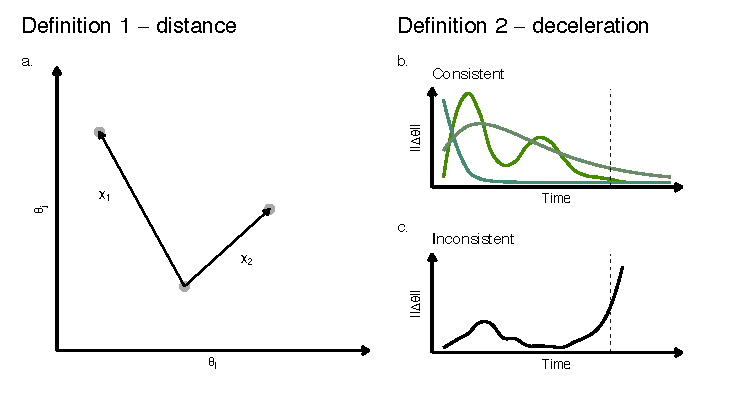
\includegraphics[width=0.95\linewidth]{img/cartoon.pdf} 
	\caption{Practical (geometric) information value, and our constraints on its dynamics. 
	\textbf{a}. This panel illustrates a two dimensional memory. The information value of two observations $\mathbf{X}_1$ and $\mathbf{X}_2$ depends on the norm of memory with learning. Here we show this distance as a euclidean norm, denoted as a black arrow.
	\textbf{b-c} This panel illustrates learning dynamics with time (over a series of observations that are not shown). If information value becomes decelerating in finite time bound, then we say that learning is consistent with Def. 2. This is shown in panel b. The bound is depicted as a dotted line. If learning does not decelerate, then it is said to be inconsistent (Panel c). \textit{It is important to note:} our account of information value and curiosity does not work when learning is inconsistent.
  	}
	\label{fig:cartoon} 
	\end{fullwidth}
\end{figure}

\subsubsection*{Bellman optimal information collection}
The common way to arrive at Bellman solution is to assume a Markov decision space. This is problem for our defition of memory, which we assume has a natural long-term path dependence. This breaks the Markov assumption, and its neeeded claim of optimal substructure. To get around this we proved that exact forgetting of the last observation is another way to achieve optimal substructure, and so to derive a Bellman solution.

 % TODO - SUBSTRUCT THEOREM HERE

Given an arbitrary starting value $E_0 > 0$, the best solution to maximizing $\hat E$ is given by Eq.~\ref{eq:V_E_bellman}. A full derivation for this fact is provided in the Appendix. 

% TODO - need the full expansion....
% DO it in Grad form....

\begin{equation}
	\label{eq:V_E_bellman} 
	V_E^{*}(\mathbf{X}) = \argmax_{\mathbf{A}} \Big [ E_0 + V_E(\mathbf{X}_1) \Big ]
\end{equation}

As long learning about the different observations $\mathbf{X}$ is independent, and as long as learning continues until steady-state, defined as $E_t < \eta$, there are many equally good solutions. Under these conditions we can simplify Eq. \ref{eq:V_E_bellman} further, giving Eq. \ref{eq:EE}. 

\begin{equation}
	\label{eq:EE} 
	V_E^{*}(\mathbf{X}) = \argmax_{\mathbf{A}} \Big [ E_t + E_{t+1} \Big ]
\end{equation}

\subsubsection*{A hypothesis about boredom}
The central failure mode of curiosity is what we'll call minutia, defined as those learning that has little to no use, ever. A good example of this is to, ``Imagine a scenario where the agent is observing the movement of tree leaves in a breeze. Since it is inherently hard to model breeze, it is even harder to predict the location of each leaf'' \cite{Pathak2017}. This will imply, they note, a curious agent will always remain curious about chaos in the leaves even though they have no hope of successful learning of them.

To limit curiosity we introduction a penalty term, $\eta$ which we treat as synomoous with boredom. We consider boredom an adaptive trait, in other words. Others have considered boredom arguing it is a useful way to motivate aversive tasks \citep{Bench2013}, or curiosity \cite{Loewenstein1994}. We take a slightly different view. We treat boredom as a tunable free parameter, $\eta \ge 0$ and a means to ignore marginal value by requiring curious exploration to stop once $E \le \eta$. 


\subsubsection*{Optimal exploration}
Having a policy $\pi_E^*$ that optomally maximizes $\hat E$ does not necessarily ensure that exploration is of good quality. We think it is reasonable to call an exploration good if it meets the criteria below. 

\begin{enumerate}
	\item Exploration should visit all available states of the environment at least once.
	\item Exploration should cease when learning has plateaued.
	\item Exploration should take as few steps as possible to achieve 1 and 2.
\end{enumerate}

In Theorems~\ref{theorem:Z} and~\ref{theorem:convergence} we prove that our Bellman solution $\pi_E$ satisfies these, when $\eta > 0$ and when the observations $\mathbf{X}$ contain complete state information, $\mathbf{S} \in \mathbf{X}$. See the Appendix for the proofs proper.

\begin{theorem}[Complete exploration] 
	\label{theorem:Z} 
	Given some arbitrary value $E_0$, an exploration policy governed by $\pi^*_{\hat E}$ will visit all states $\mathbf{S} \in \mathbb{S}$ in finite number of steps $T$.
\end{theorem}

\begin{theorem}[Efficient exploration] 
	\label{theorem:convergence} 
	An exploration policy governed by $\pi^*_{\hat E}$ will only revisit states for where information value is marginally useful, defined by $\hat E > \eta$.  
\end{theorem}


\subsubsection*{A hypothesis of equal importance}
 Searching in an open-ended way for information must be less efficient than a direct search for reward? In answer to this question, we make two conjectures.

\begin{conjecture}[A hypothesis of equal importance]
	Reward value and information value are equally important for survial, in changing environments 
\end{conjecture}

It's worth reiterating here, that curiosity is a primary drive in most, if not all, animals \cite{Inglis2001}. It is as strong, if not sometimes stronger, than the drive for reward \cite{Loewenstein1994,Kidd2015,Gottlieb2018}.

If both reward and information are equally important, then time is not wasted in a curious search, and so the process is not \textit{necessarily} inefficient or even indirect. Instead, we offer a new question. Is curiosity practical enough to serve as a useful ``trick'' to solve reward collection search problems? We answer this with a second conjecture,

\begin{conjecture}[The curiosity trick]
	When learning is possible, curiosity is a sufficient solution for all exploration problems.
\end{conjecture}

It's worth noting here that curiosity, as an algorithm in machine learning, is highly effective at solving broad kinds of optimization problems \cite{Schmidhuber1991,Stanton2018,Lehman2010,Mouret2011,Fister2019,Mouret2015,Colas2020,Cully2015,Pathak2017,Laversanne-Finot2018}. 

\subsubsection*{The problem of mixing reward and information collection}
If reward and information are equally important, and curiosity is sufficient, how can an animal go about balancing them? If you accept our conjectures, then answering this question optimally is the same as solving the dilemma. To solve this dual value learning problem we’ve posed–-information and reward maximization–-we need an algorithm that can maximize the value of a mixed sequence, $V_{\hat{E}R}$. For example,

\begin{equation}
	\label{eq:bellman_seq_ER}
	V^*_{\hat{E}R}(\mathbf{S}) = \argmax_{\mathbf{A} \in \mathbb{A}} \Big [\sum_{k=0}^{T} \hat{E}_t + \hat{E}_{t+1} + R_{t+2} + \hat{E}_{t+3} + R_{t+4} + \ldots  \ \Big ]
\end{equation}

\subsubsection*{A win-stay, lose-switch solution}
A similar dual value optimization problem to Eq.~\ref{eq:bellman_seq_ER} was posed, solved, with its regret bounded, by Robbins \cite{Robbins1952} in his derivation of the win-stay lose-swtich rule. This WLSL approach has since proven uesful in decision making and reinforcement learning \cite{Estes1994TowardAS,Worthy2014}, Bayesian sampling \cite{Bonawitz2014}, and especially in game theory \cite{Nowak1993}. We also put it to use here. 

We have come to think about our two optimal value policies $\pi_R$ and $\pi_{\hat E}$ as two ``players'' in game for behavioral control of an animal's moment-by-moment actions \cite{Estes1994TowardAS}. The simplest solution to this game, in terms computational complexity, is a WSLS rule. We denote this rule as $\Pi_\pi$, and define it here by a set of inequalities,

\begin{equation} 
    \label{eq:pipi}
    \begin{split}
        \Pi_{\pi} = 
        \begin{cases}
            \pi^*_{\hat{E}} & : \hat{E} - \eta > R + \rho \\
            \pi_R 	& : \hat{E} - \eta < R + \rho \\
        \end{cases}
    \end{split}
\end{equation}

Here $eta$ is the boredom tern we defined earlier. We also introduce the reward bias term $\rho$, where $\rho > \eta$. This bias ensures no ties can occur, and that as $\hat E$ decreases to 0, as it must, the default policy is reward collection. That is, by $\pi_R$.

In Eq.~\ref{eq:pipi} we compare reward $R$ and information value $\hat E$ but have not made sure they have same ``units'', or are otherwise comparible. We sidestep this isssue by limiting the probability of having zero reward to be, itself, non-zero. That is, $p(R_t=0) > 0$. We also limit $E_0$, the first set of values, to be positive and non-zero when used with boredom, $(E_0 - \eta) > 0$. These constraints ensure complete ``good'' exploration (defined above),which in turn ensures optimal reward learning is possible irrespitive of the reltative scales of $R$ and $\hat E$.

To provide some intuition for Eq.\ref{eq:pipi}, imagine that in the previous action an animal observed, arbitrarily, 0.7 units of information value, $\hat E$, and no reward (i.e. $R = 0$). Using our rule on the next action the animal should then choose its exploration policy $\pi^*_{\hat{E}}$. If it explored last time, this is a ``stay'' action. If not, it is a ``swtich''. Let's then say that with this next observation, $\hat E$ decreases to 0.2 and a reward value of 1.0 is observed. Now the animals should swtich its strategy for the next round, to exploit instead. 

In general, if there was more reward value then information value last round ($R > \hat E$), our rule dictates an animal should choose the reward policy. If information value dominated, $R < \hat E$, then it should choose the information gathering policy.

The WSLS rule in Eq~\ref{eq:pipi} when applied to exploration-exploitation problems can gauentee three things, shown below. 

\begin{theorem}[No regret - reward value]
	\label{th:no_regret_R}
	When $\pi_R$ is in control under $\Pi_{\pi}$, all actions are zero regret in terms of $V_R$. That is, $\sum_{k=0}^{T} G = 0$.
\end{theorem}

\begin{theorem}[No regret - information value]
	\label{th:no_regret_E}
	When $\pi_{\hat E}$ is in control under $\Pi_{\pi}$, all actions are zero regret in terms of $V_{\hat E}$. That is, $\sum_{k=0}^{T} G = 0$.
\end{theorem}

\begin{theorem}[No regret - mixed values]
	\label{th:no_regret_ER}
	When either $\pi_{\hat E}$ or $\pi_R$ is in control under $\Pi_{\pi}$, all actions are zero regret in terms of $V_{\hat{E}R}$. That is, $\sum_{k=0}^{T} G = 0$.
\end{theorem}

In each of theses Theoreums we assume our definitions for $\mathbf{X}$, $\mathbf{A}$, $\mathbf{M}$, $f$, $\Lambda$, and $\Pi_{\pi}$ are implicitly given, and a finite horizon $T$. Proofs for Theorems~\ref{th:no_regret_E} and~\ref{th:no_regret_E} follow from both reinforcement learning and our definition of information optimization having a Bellman optimality. The proof for the optimality of $V_{\hat{E}R}$ (Th~\ref{th:no_regret_ER}) in provided in the Appendix. The intuition for this proof is simple that a greedy algorithm made over two Bellman solutions is itself a Bellman solution.

In Eq.~\ref{eq:pipi} we compare reward $R$ and information value $\hat E$ but have not ensured they have same ``units'', or are comparible valuables. We sidestep this isssue by limiting the probability of having zero reward to be, itself, non-zero. That is, $p(R_t=0) > 0$. We also limit $E_0$, the first set of values, to be positive and non-zero when used with boredom, $(E_0 - \eta) \geq 0$. These constraints ensure complete ``good'' exploration (defined above) which in turn ensures optimal reward learning is possible.

\subsubsection*{Homeostasic adjustments}
We have been studying cases where reward value is fixed. That is, where environment reward $R$ is equal to its subjective value to the animal, $\hat R$. In natural behavior though the motivational value of reward often declines as the animal reaches satiety \citep{Keramati2014,Juechems2019,Munch2020}. This is called reward homeostatsis. Fortunately, it has been shown a reward collection policy designed for one style will work for the other \citep{Keramati2014}. However to use a form similiar to Eq. \ref{eq:pipi} for the dilemmaa under homeostatic reward value, we need to make one modification. This is shown in Eq.~\ref{eq:pipi_h}. 

\begin{equation} 
    \label{eq:pipi_h}
    \begin{split}
        \Pi_{\pi} = 
        \begin{cases}
            \pi^*_{\hat{E}} & : \hat{E} - \eta > R - \rho \\
            \pi_R 	& : \hat{E} - \eta < R - \rho \\
        \end{cases}
    \end{split}
\end{equation}

Under homeostasis ties between values in Eq. \ref{eq:pipi} should be broken in favor of exploration, because if exploitation remains the defualt, reward homeostasis is not possible. 

% ----------------------------------------------------------------------
\subsection*{Experiments}
Does our theory work in practice? Our approach does not mathematically ensure a mixed value solution to explore-exploit problems will always maximizes reward value, comparerd with other well-established methods. The remainder of this paper is devoted to studying our approaches performance in simulated bandit tasks. Each task was designed to either test exploration performance in a way that matches recent experimental studies, or to test the limits of curiosity. 

\subsubsection*{Information collection}
The work so far has built up the idea that the most valuable, and most efficient, curious search will come from a deterministic algorithm. That is, every step strictly maximizes $\hat E$. It is this determinism which will let us resolve the dilemma, later on. A deterministic view of exploration seems at odds with how the problem is generally viewed today, which involves searching with some amount of randomness. Whereas if our analysis is correct, randomness is not needed or desirable, as it must lead to less value and a longer search. 

We confirm and illustrate this result using an example of a simple information foraging task (Task 1; Fig.\label{fig:task_outline1}). This variation of the bandit task \citep{Sutton2018} replaces rewards with information, in this case colors. On each selection, the agent sees one of two colors according to a specific probability shown in Fig. ~\ref{fig:payout}a. When the relative color probabilities are more similar that arm has more entropy and so more to learn and more information value. Arms that are certain to present only one color lose their informative value quickly.

The results of this simple information seeking task are shown in Figure~\ref{fig:curiosity1}. Deterministic curiosity in this task generated more information value, in less time, and with zero regret when compared against a stochastic agent using more directed random search. As our work here predicts, noise only made the search happen slower and lead to regret. Besides offering a concrete example, performance in Task 1 is a first step in showing that even though $\pi_E$'s optimality is proven for a deterministic environment, it can perform well in other settings.

\begin{figure}
	\begin{fullwidth}
	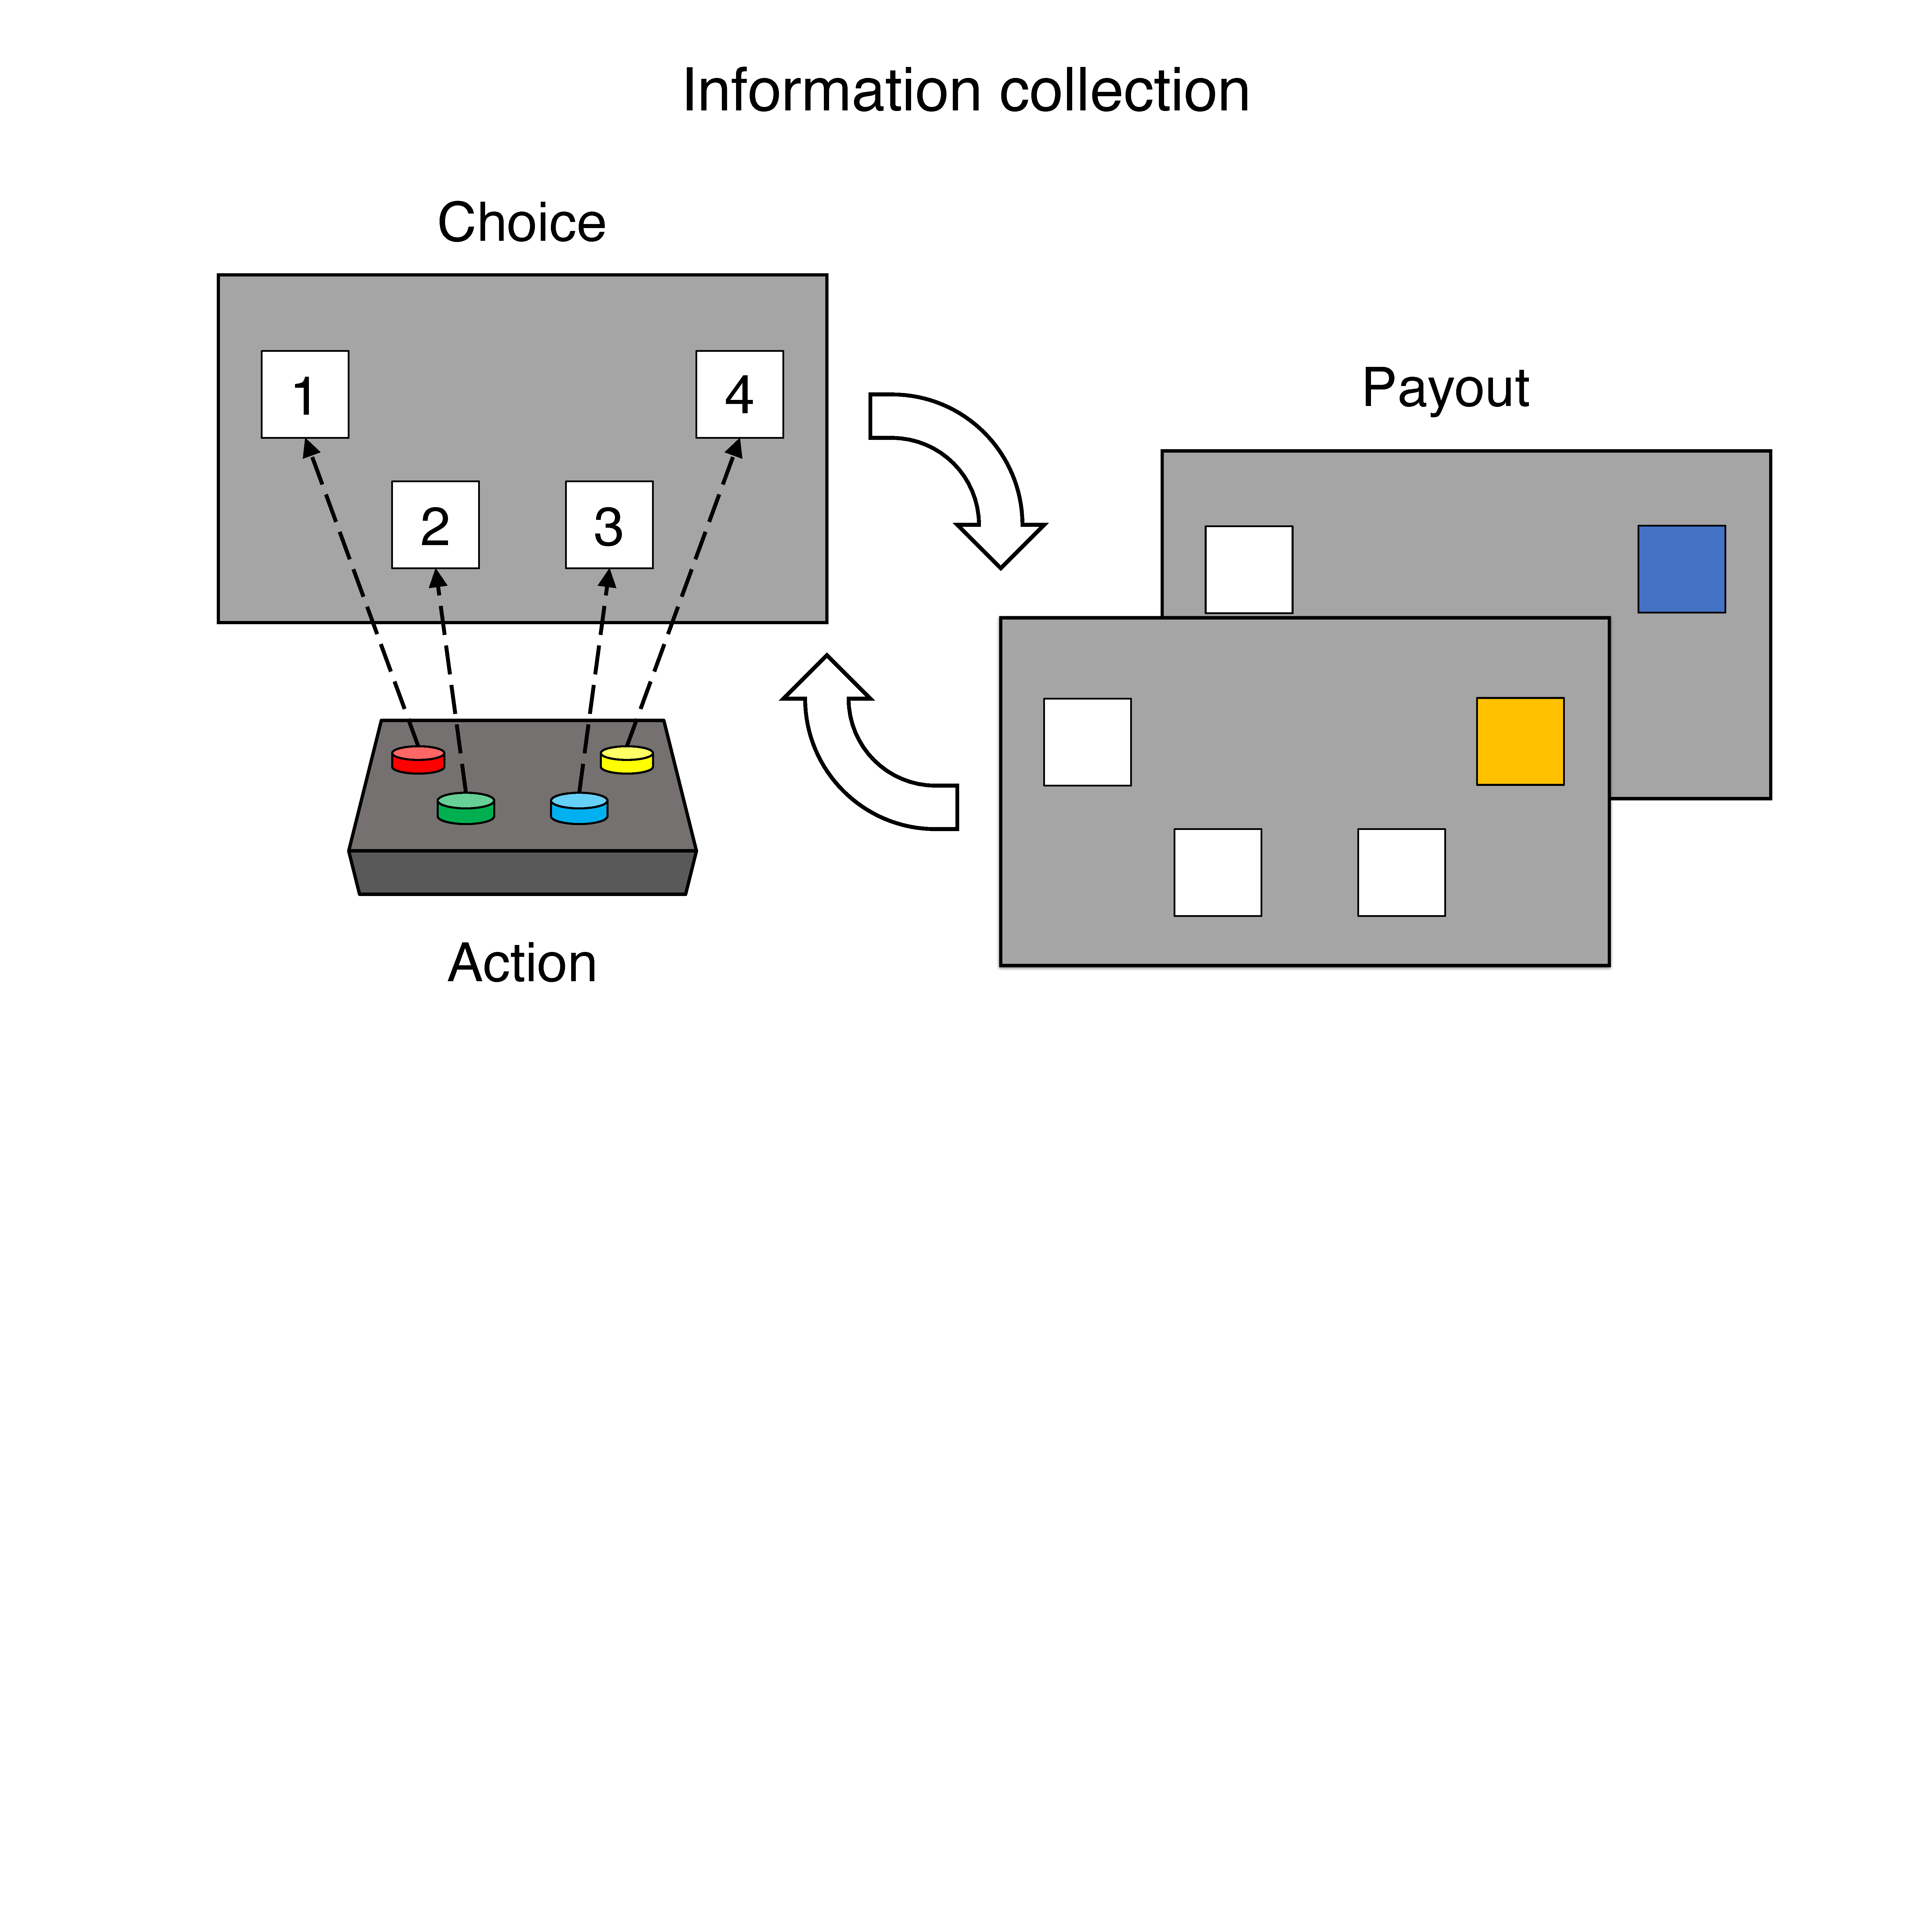
\includegraphics[width=1.0\linewidth]{img/task_outline1.pdf} 
	\caption{A simple four choice information foraging task. The information in this task is a yellow or blue stimulus, which can change from trial to trial. A good learner in this task is one who tries to learn the probabilities of all the symbols in each of the four choices. The more random the stimuli are in a choice, the more potential information/entropy there is to learn. \textit{Note}: the information payout structure is shown below (Fig.~\ref{fig:payout}a}).
	\label{fig:task_outline1} 
	\end{fullwidth}
\end{figure}

\begin{figure}
	\begin{fullwidth}
	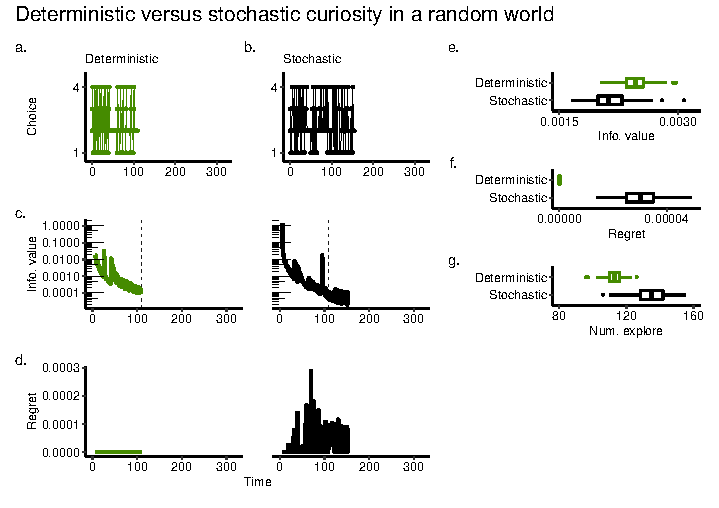
\includegraphics[width=1.0\linewidth]{img/curiosity1.pdf} 
	\caption{Comparing deterministic versus stochastic variations of the same curiosity algorithm, in a simple information foraging task (Task 1). Deterministic results are shown in the left column, and stochastic are shown in the right. The hyperparameters for both models were found by random search, which is described in the Methods.
	\textbf{a-b}. Examples of choice behavior.
	\textbf{c-d}. Information value plotted with time for the behavior shown in a-b.
	\textbf{e-f}. Regret plotted with time for the behavior shown in a-b. Note how our only deterministic curiosity generates zero regret, inline with theoretical predictions.
	\textbf{e}. Average information value for 100 independent simulations. Large values mean a more efficient search.
	\textbf{f}. Average regret for 100 independent simulations. Ideal exploration should have no regret. 
	\textbf{g}. Number of steps it took to reach the boredom threshold $eta$. Smaller values imply a faster search.
	}
	\label{fig:curiosity1} 
	\end{fullwidth}
\end{figure}


\subsubsection*{Reward collection} 
Our approach does not mathematically ensure a dual value solution to the dilemma maximizes reward value comparerd with other well-established methods. To findout we meaasured total reward collected over 7 tasks and 10 agents, including ours. Each agent's parameters were independently optimized for each task. For a brief description of each agent, see Table~\ref{tab:agents}. They all have in common that their central goal is to maximize total reward value, though this is often supplemented by some other goal, an intrinic reward or bonus \cite{Ng1999,Sutton1998}. 

The general form of the 7 tasks are depicted in Fig~\ref{fig:task_outline2}. As with our first task (Fig. ~\ref{fig:task_outline1}) they are all variations of the classic multi-armed bandit \citep{Sutton2018}. The payouts for each of the tasks are shown separately in Fig.~\ref{fig:payout}. Every trial has a set of $n$ choices. Each choice returns a “payout”, according to a predetermined probability. Payouts are information, a reward, or both. Note that, as in Task 1, information was symbolic, denoted by a color code, “yellow” and “blue” and as is custom reward was a positive real number. 

The results in full for all tasks and exploration strategies are shown in Fig.~\ref{fig:summary}. All agents, including ours, used the same exploitation policy based on the temporal difference learning rule \citep{Sutton2018} (Methods).

\begin{figure}
	\begin{fullwidth}
	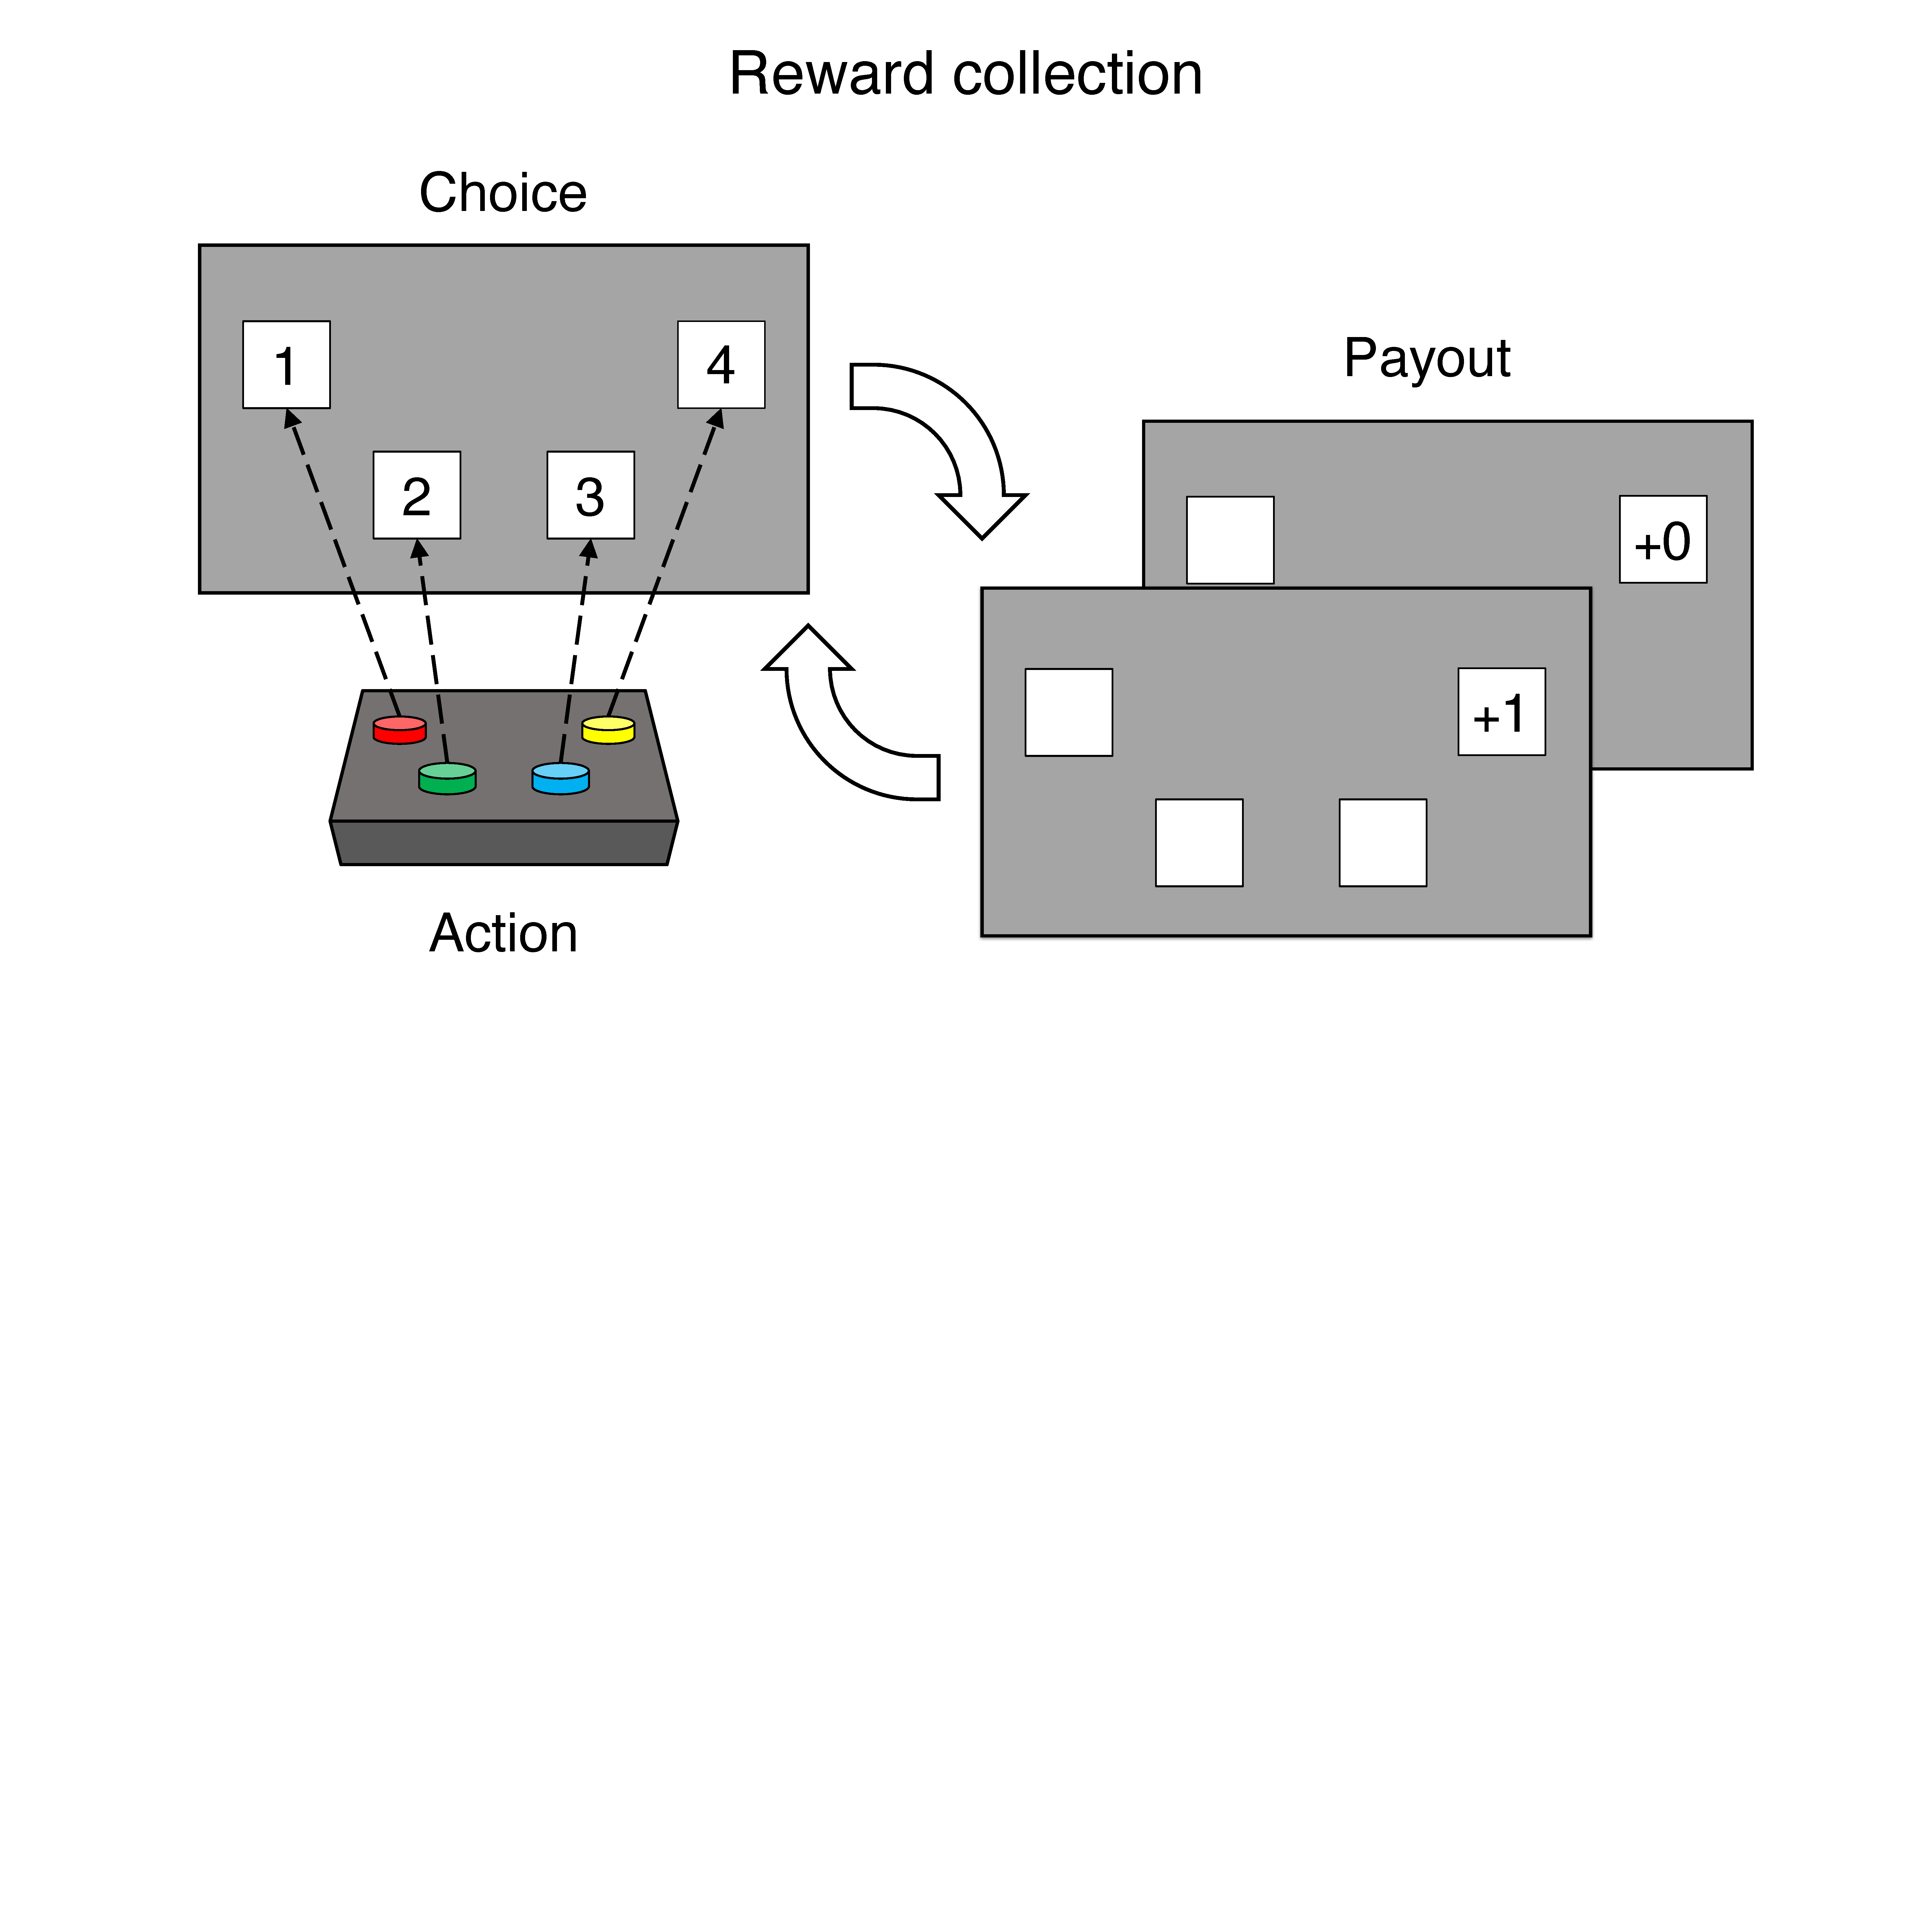
\includegraphics[width=1.0\linewidth]{img/task_outline2.pdf} 
	\caption{A 4 choice reward collection task. The reward is numerical value, here a 1 or 0. A good learner in this task is one who collects the most rewards. The task depicted here matches that in Fig~\ref{fig:payout}b. Every other reward collection task we study has the same basic form, only the number of choices increases and the reward spaces are more complex.}
	\label{fig:task_outline2} 
	\end{fullwidth}
\end{figure}

\begin{figure}
	\begin{fullwidth}
	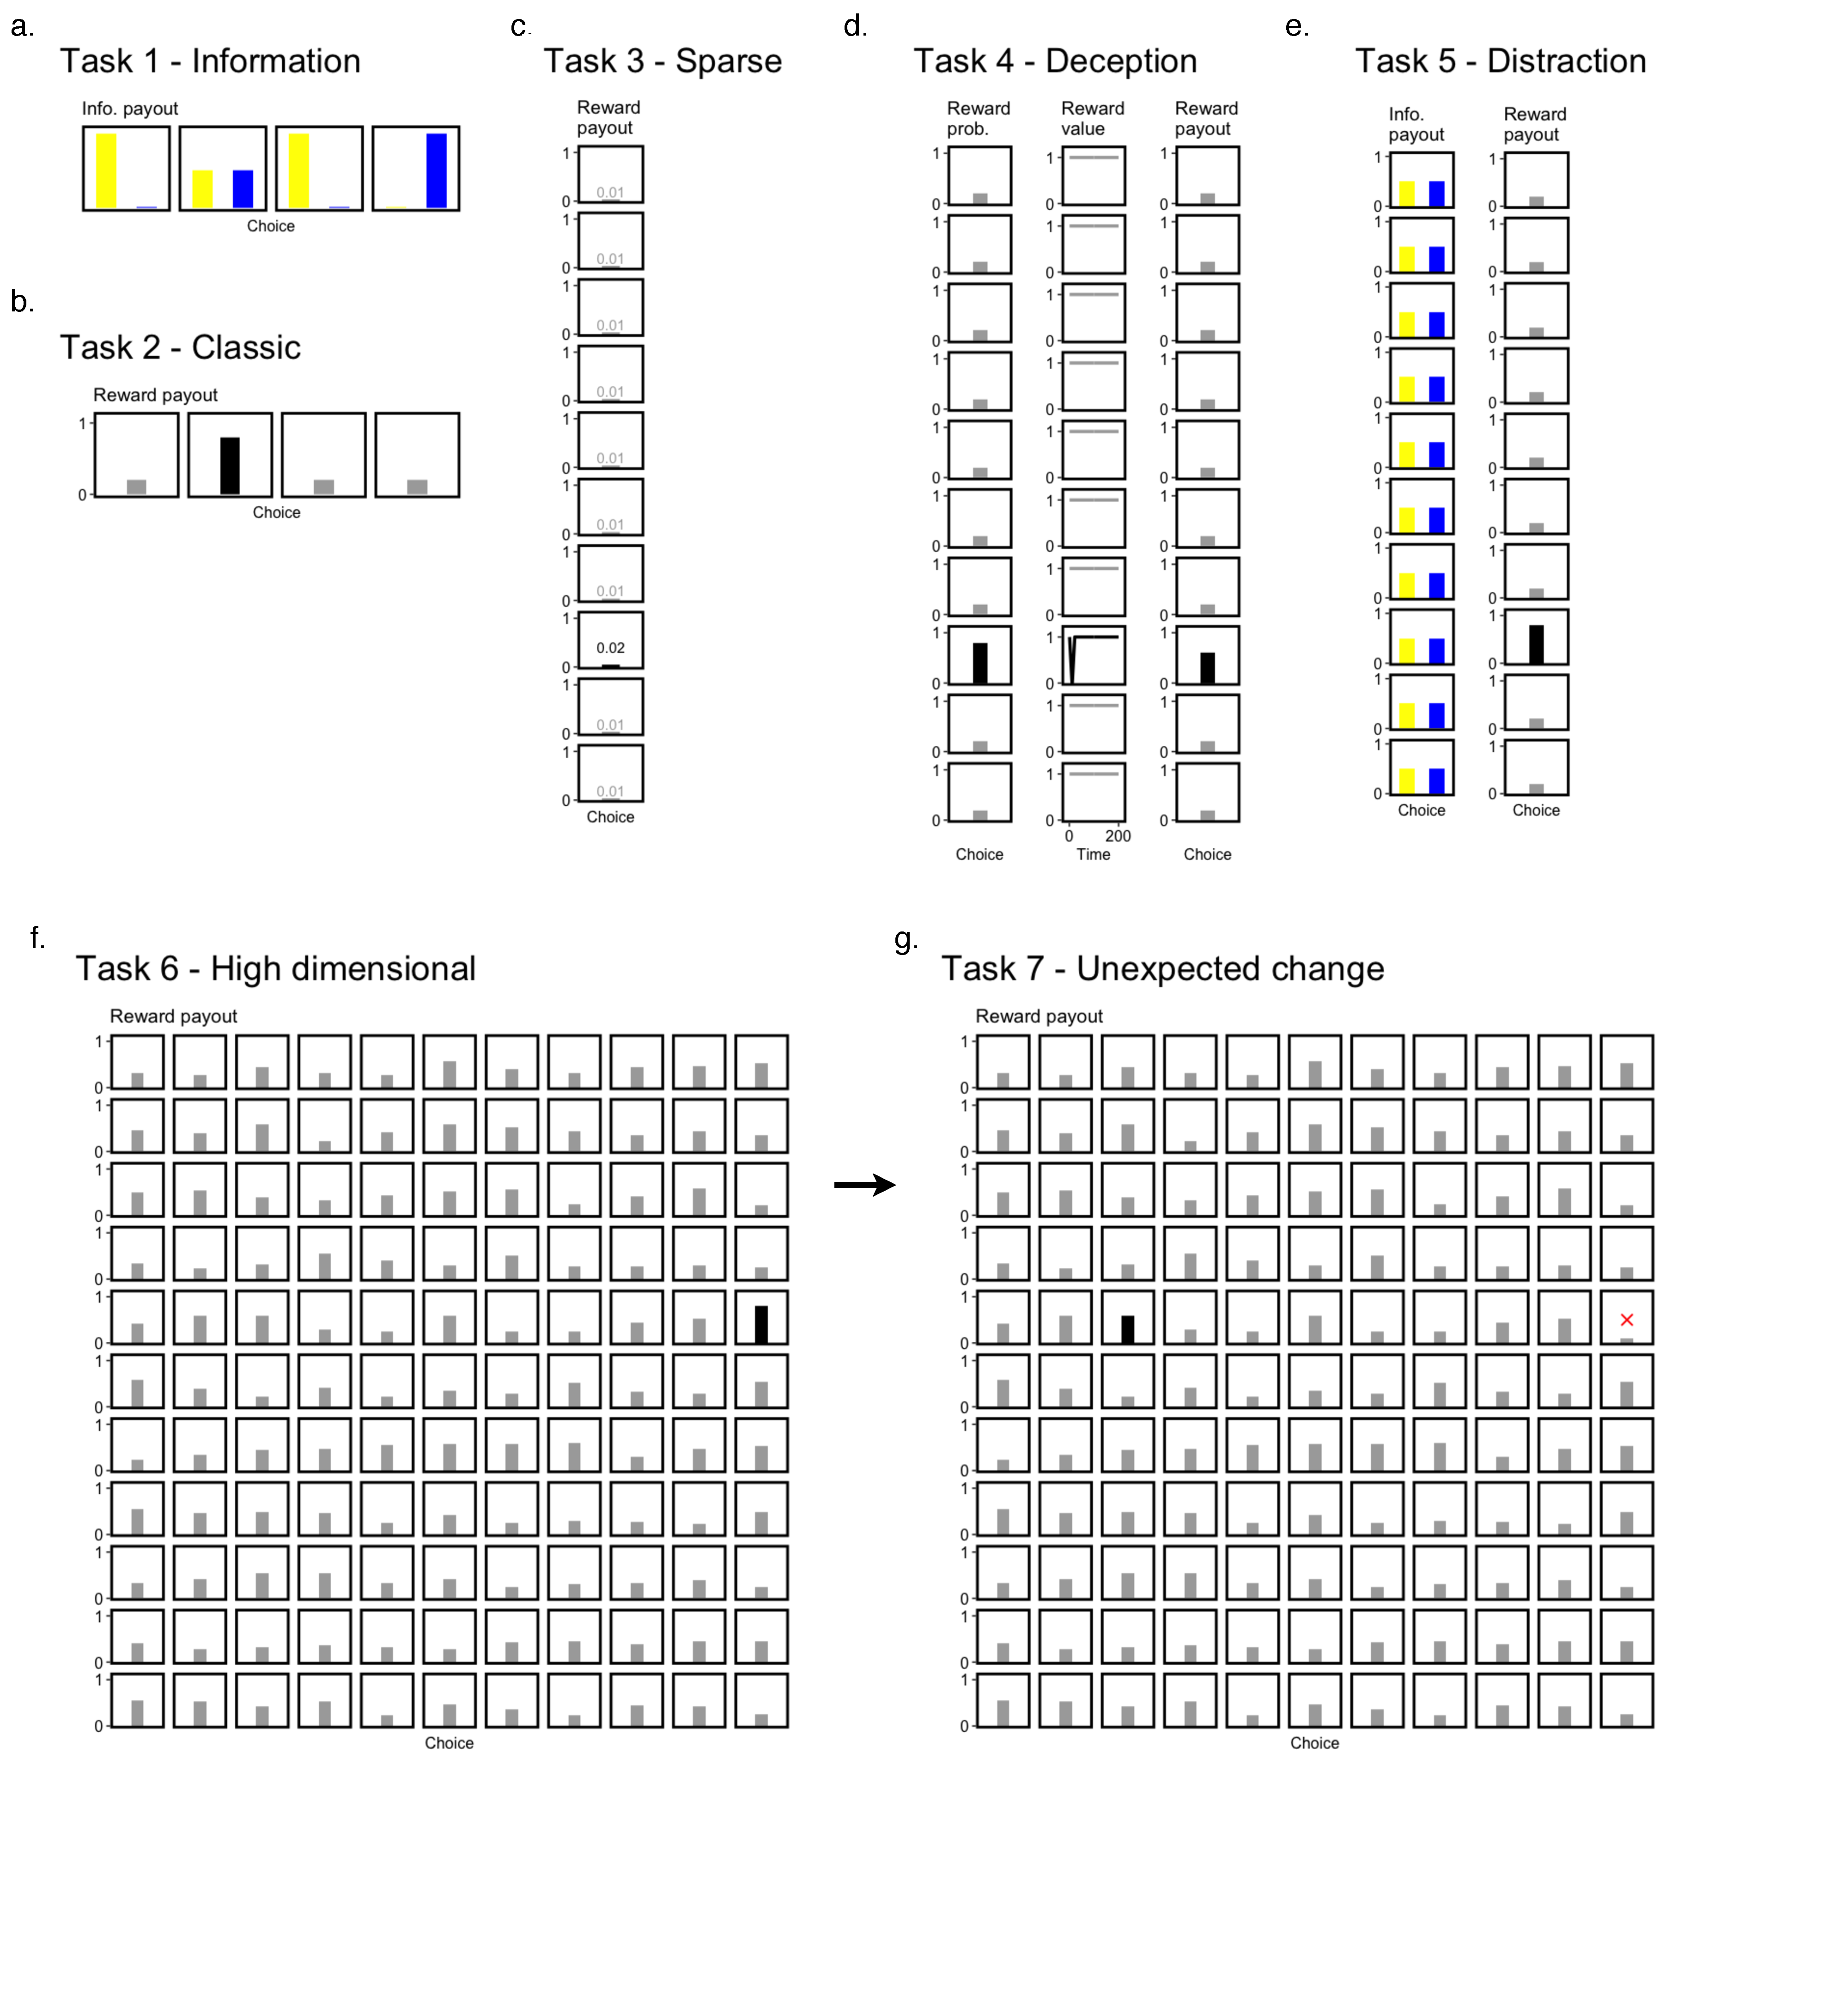
\includegraphics[width=0.95\linewidth]{img/task_payout.pdf} 
	\caption{Payouts for \textit{Tasks 1 - 7}. Payouts can be information, reward, or both. For comments on general task design, see Fig~\ref{fig:task_outline2}.
	\textbf{a.} A classic four-choice design for information collection. A good learner should visit each arm, but quickly discover that only arm two is information bearing.
	\textbf{b.} A classic four-choice design for testing exploration under reward collection. The learner is presented with four choices and it must discover which choice yields the highest average reward. In this task that is Choice 2. 
	\textbf{c.} A ten choice sparse reward task. The learner is presented with four choices and it must discover which choice yields the highest average reward. In this task that is Choice 8 but the very low overall rate of rewards makes this difficult to discover. Solving this task with consistency means consistent exploration. 
	\textbf{d.} A ten choice deceptive reward task. The learner is presented with 10 choices, but the choice which is the best on the long-term (>30 trials) has a lower value in the short term. This value first declines, then rises (see column 2).
	\textbf{e.} A ten choice information distraction task. The learner is presented with both information and rewards. A good learner though will realize the information does not predict reward collection, and so will ignore it.
	\textbf{f.} A 121 choice task with a complex payout structure. This task is thought to be at the limit of human performance. A good learner will eventually discover choice number 57 has the highest payout.
	\textbf{g.} This task is identical to \textit{a.}, except for the high payout choice being changed to be the lowest possible payout. This task tests how well different exploration strategies adjust to simple but sudden change in the environment.
	}
	\label{fig:payout} 
	\end{fullwidth}
\end{figure}

\begin{table}[]
	\caption{Exploration strategies.}
	\label{tab:agents}
	\begin{tabular}{|l|l|l|}
	\hline
	\textbf{Name} & \textbf{Class} & \textbf{Exploration strategy} \\ \hline
	Curiosity & Deterministic & Maximize information value \\ \hline
	Random/Greedy & Random & \begin{tabular}[c]{@{}l@{}}Alternates between random exploration \\ and greedy with probability $\epsilon$.\end{tabular} \\ \hline
	Decay/Greedy & Random & \begin{tabular}[c]{@{}l@{}}The $\epsilon$ parameter \\ decays with a half-life $\tau$\end{tabular} \\ \hline
	Random & Random & Pure random exploration \\ \hline
	Reward & Extrinsic & Softmax sampling of reward value \\ \hline
	Bayesian & Extrinsic + Intrinsic & Sampling of reward value + information value \\ \hline
	Novelty & Extrinsic + Intrinsic & Sampling of reward value + novelty signal \\ \hline
	Entropy & Extrinsic + Intrinsic & Sampling of reward value + action entropy \\ \hline
	Count (EB) & Extrinsic + Intrinsic & Sampling of reward value + visit counts \\ \hline
	Count (UCB) & Extrinsic + Intrinsic & Sampling of reward value + visit counts \\ \hline
	\end{tabular}
\end{table}

\begin{figure}
    \label{fig:summary} 
	\begin{fullwidth}
	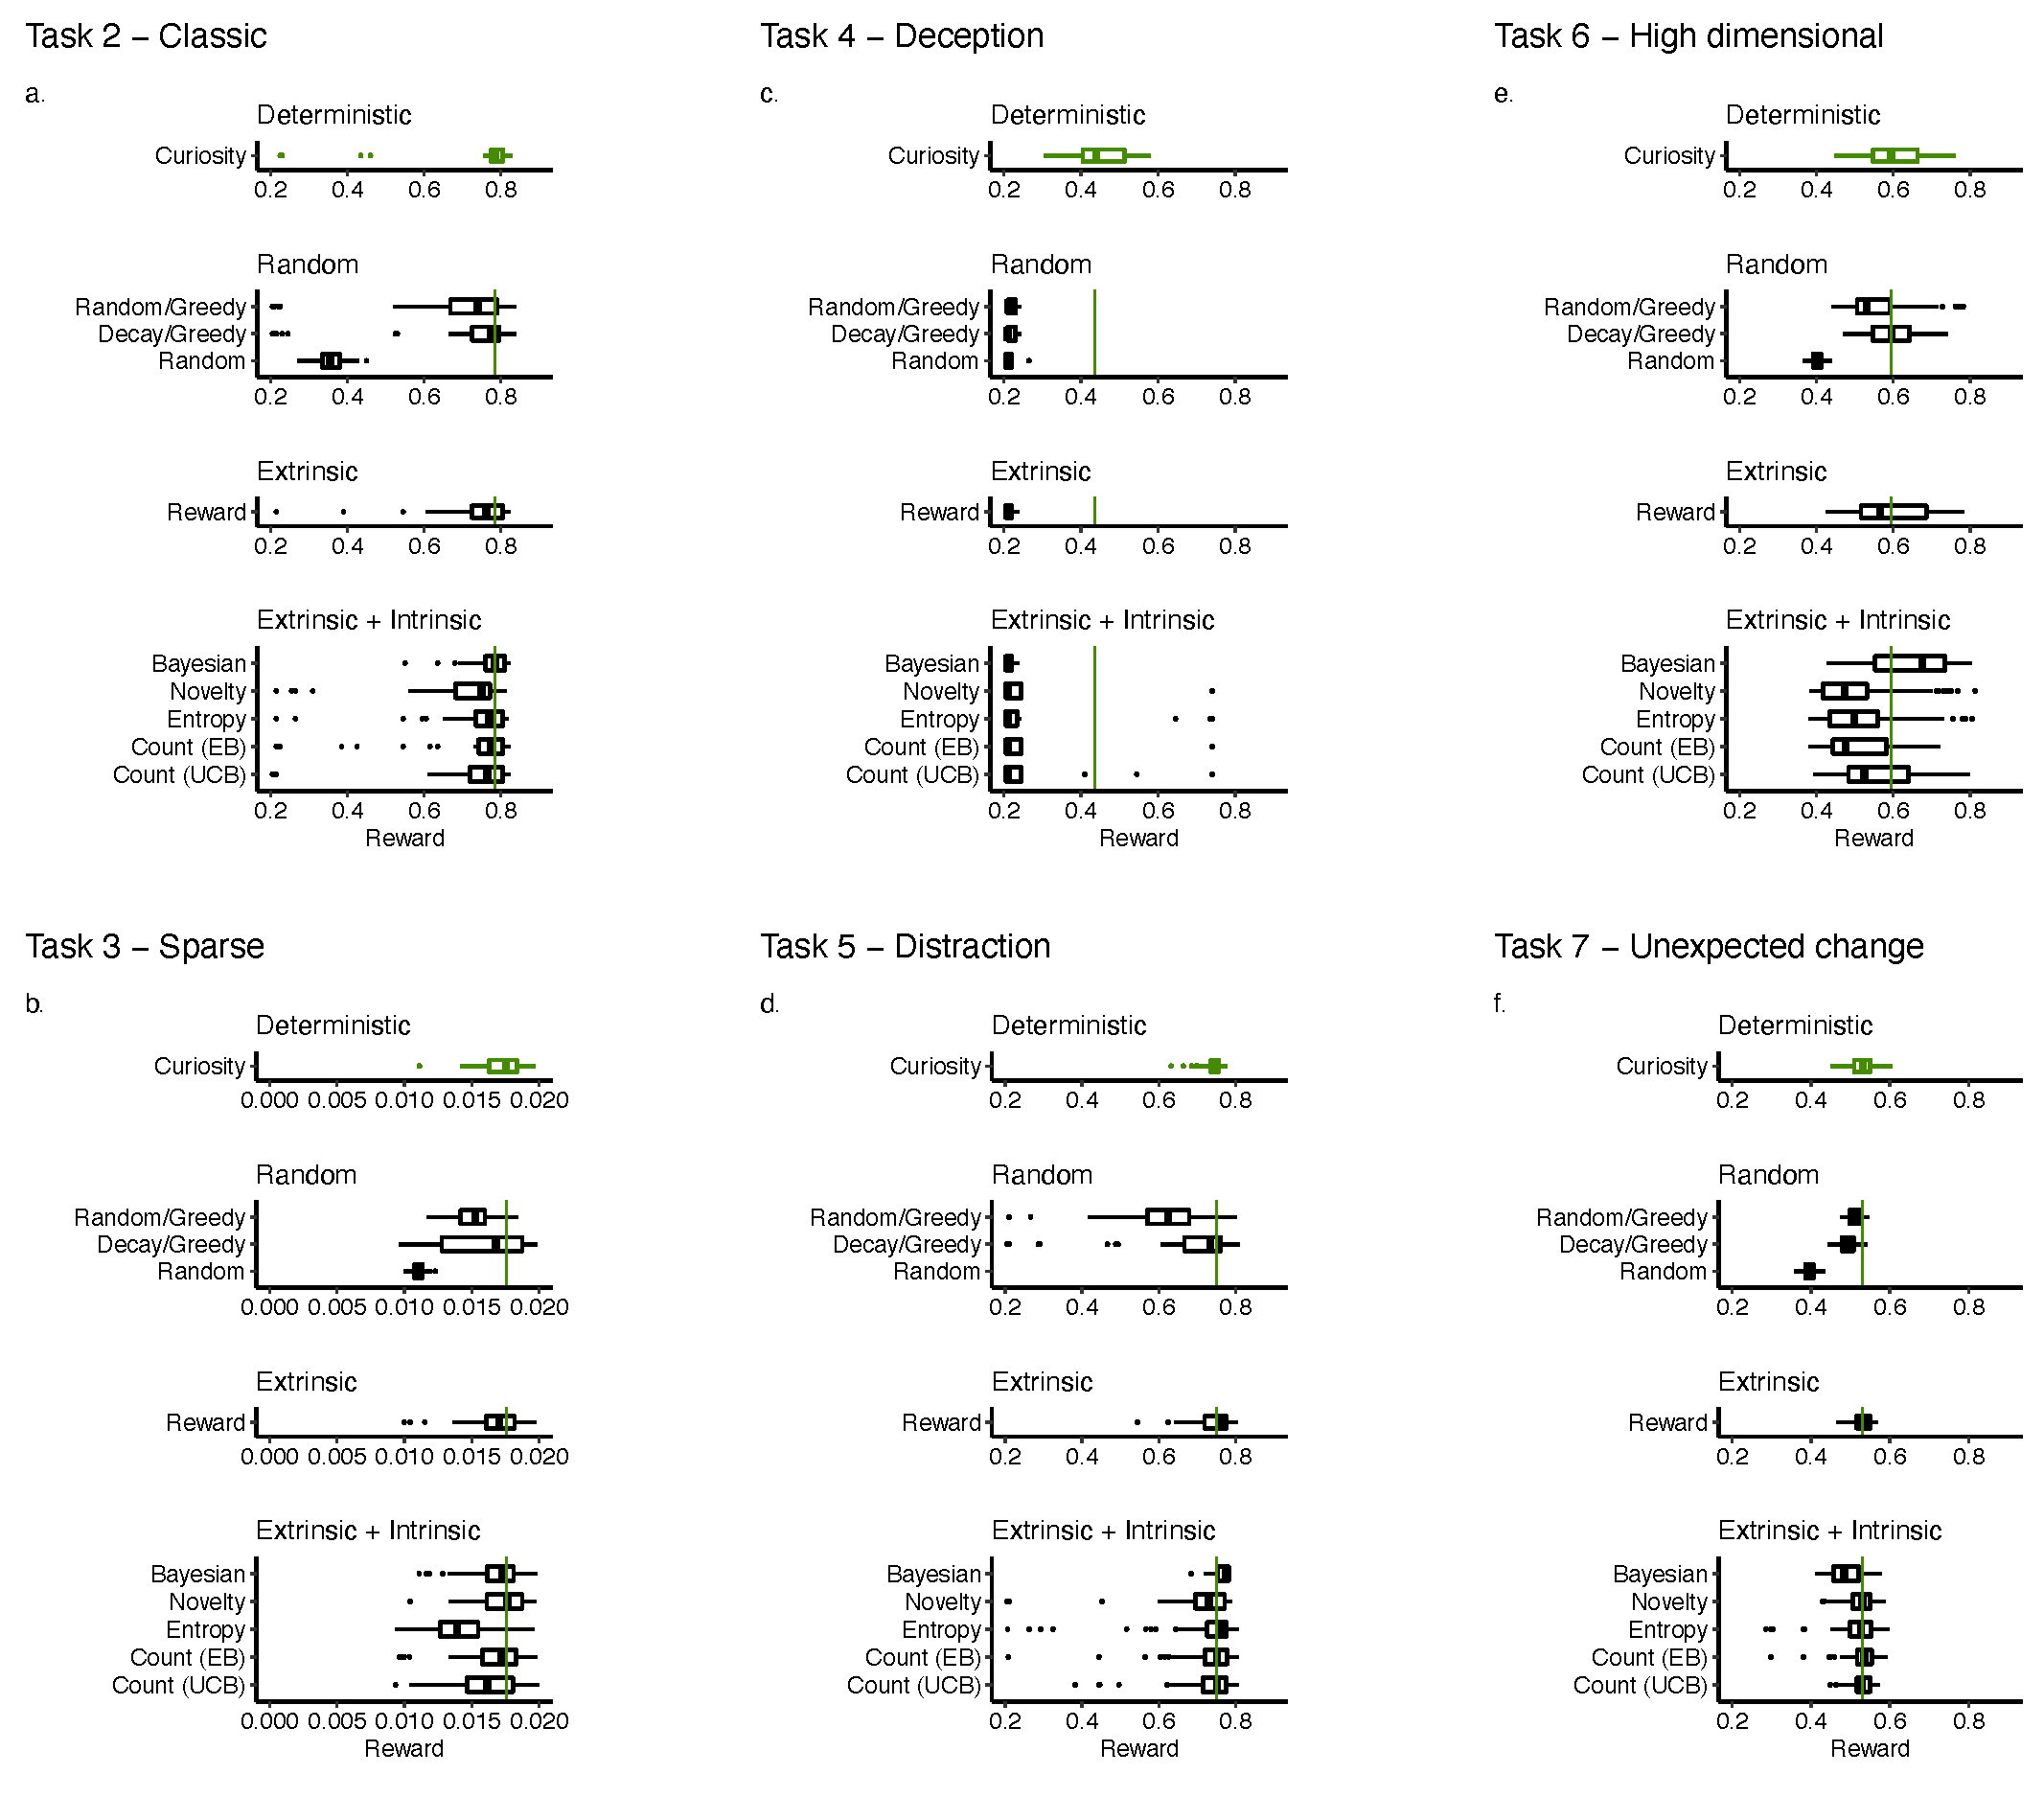
\includegraphics[width=1\linewidth]{img/summary.pdf} 
	\caption{Summary of reward collection (\textit{Tasks 2-7}). The strategies in each panel are grouped according to the class of search they employed (Curiosity. Random, Extrinsic reward or Extrinsic + Intrinsic rewards). 
	\textbf{a.} Results for Task 2, which has four choices and one clear best choice.
	\textbf{b.} Results for Task 3, which has 10 choices and very sparse positive returns.
	\textbf{c.} Results for Task 4, whose best choice is initially ``deceptive'' in that it returns suboptimal reward value over the first 20 trials.
	\textbf{d.} Results for Task 5, which blends the information foraging task 1 with a larger version of Task 2. The yellow/blue stimuli are a max entropy distraction which do not predict the reward payout of each arm.
	\textbf{e.} Results for Task 6, which has 121 choices and a quite heterogeneous set of payouts but still with one best choice.
	\textbf{f.} Results for Task 7, which is identical to Task 6 except the best choice was changed to be the worst. The learners from Task 6 were trained on this Task beginning with the learned values from their prior experience -- a test of robustness to sudden change in the environment. 
	\textit{Note}: To accommodate the fact that different tasks were run different numbers of trials, we normalized total reward by trial number. This lets us plot reward collection results for all tasks on the same scale.
  	}
	
	\figsupp{Summary of regret (\textit{Tasks 2-7})}{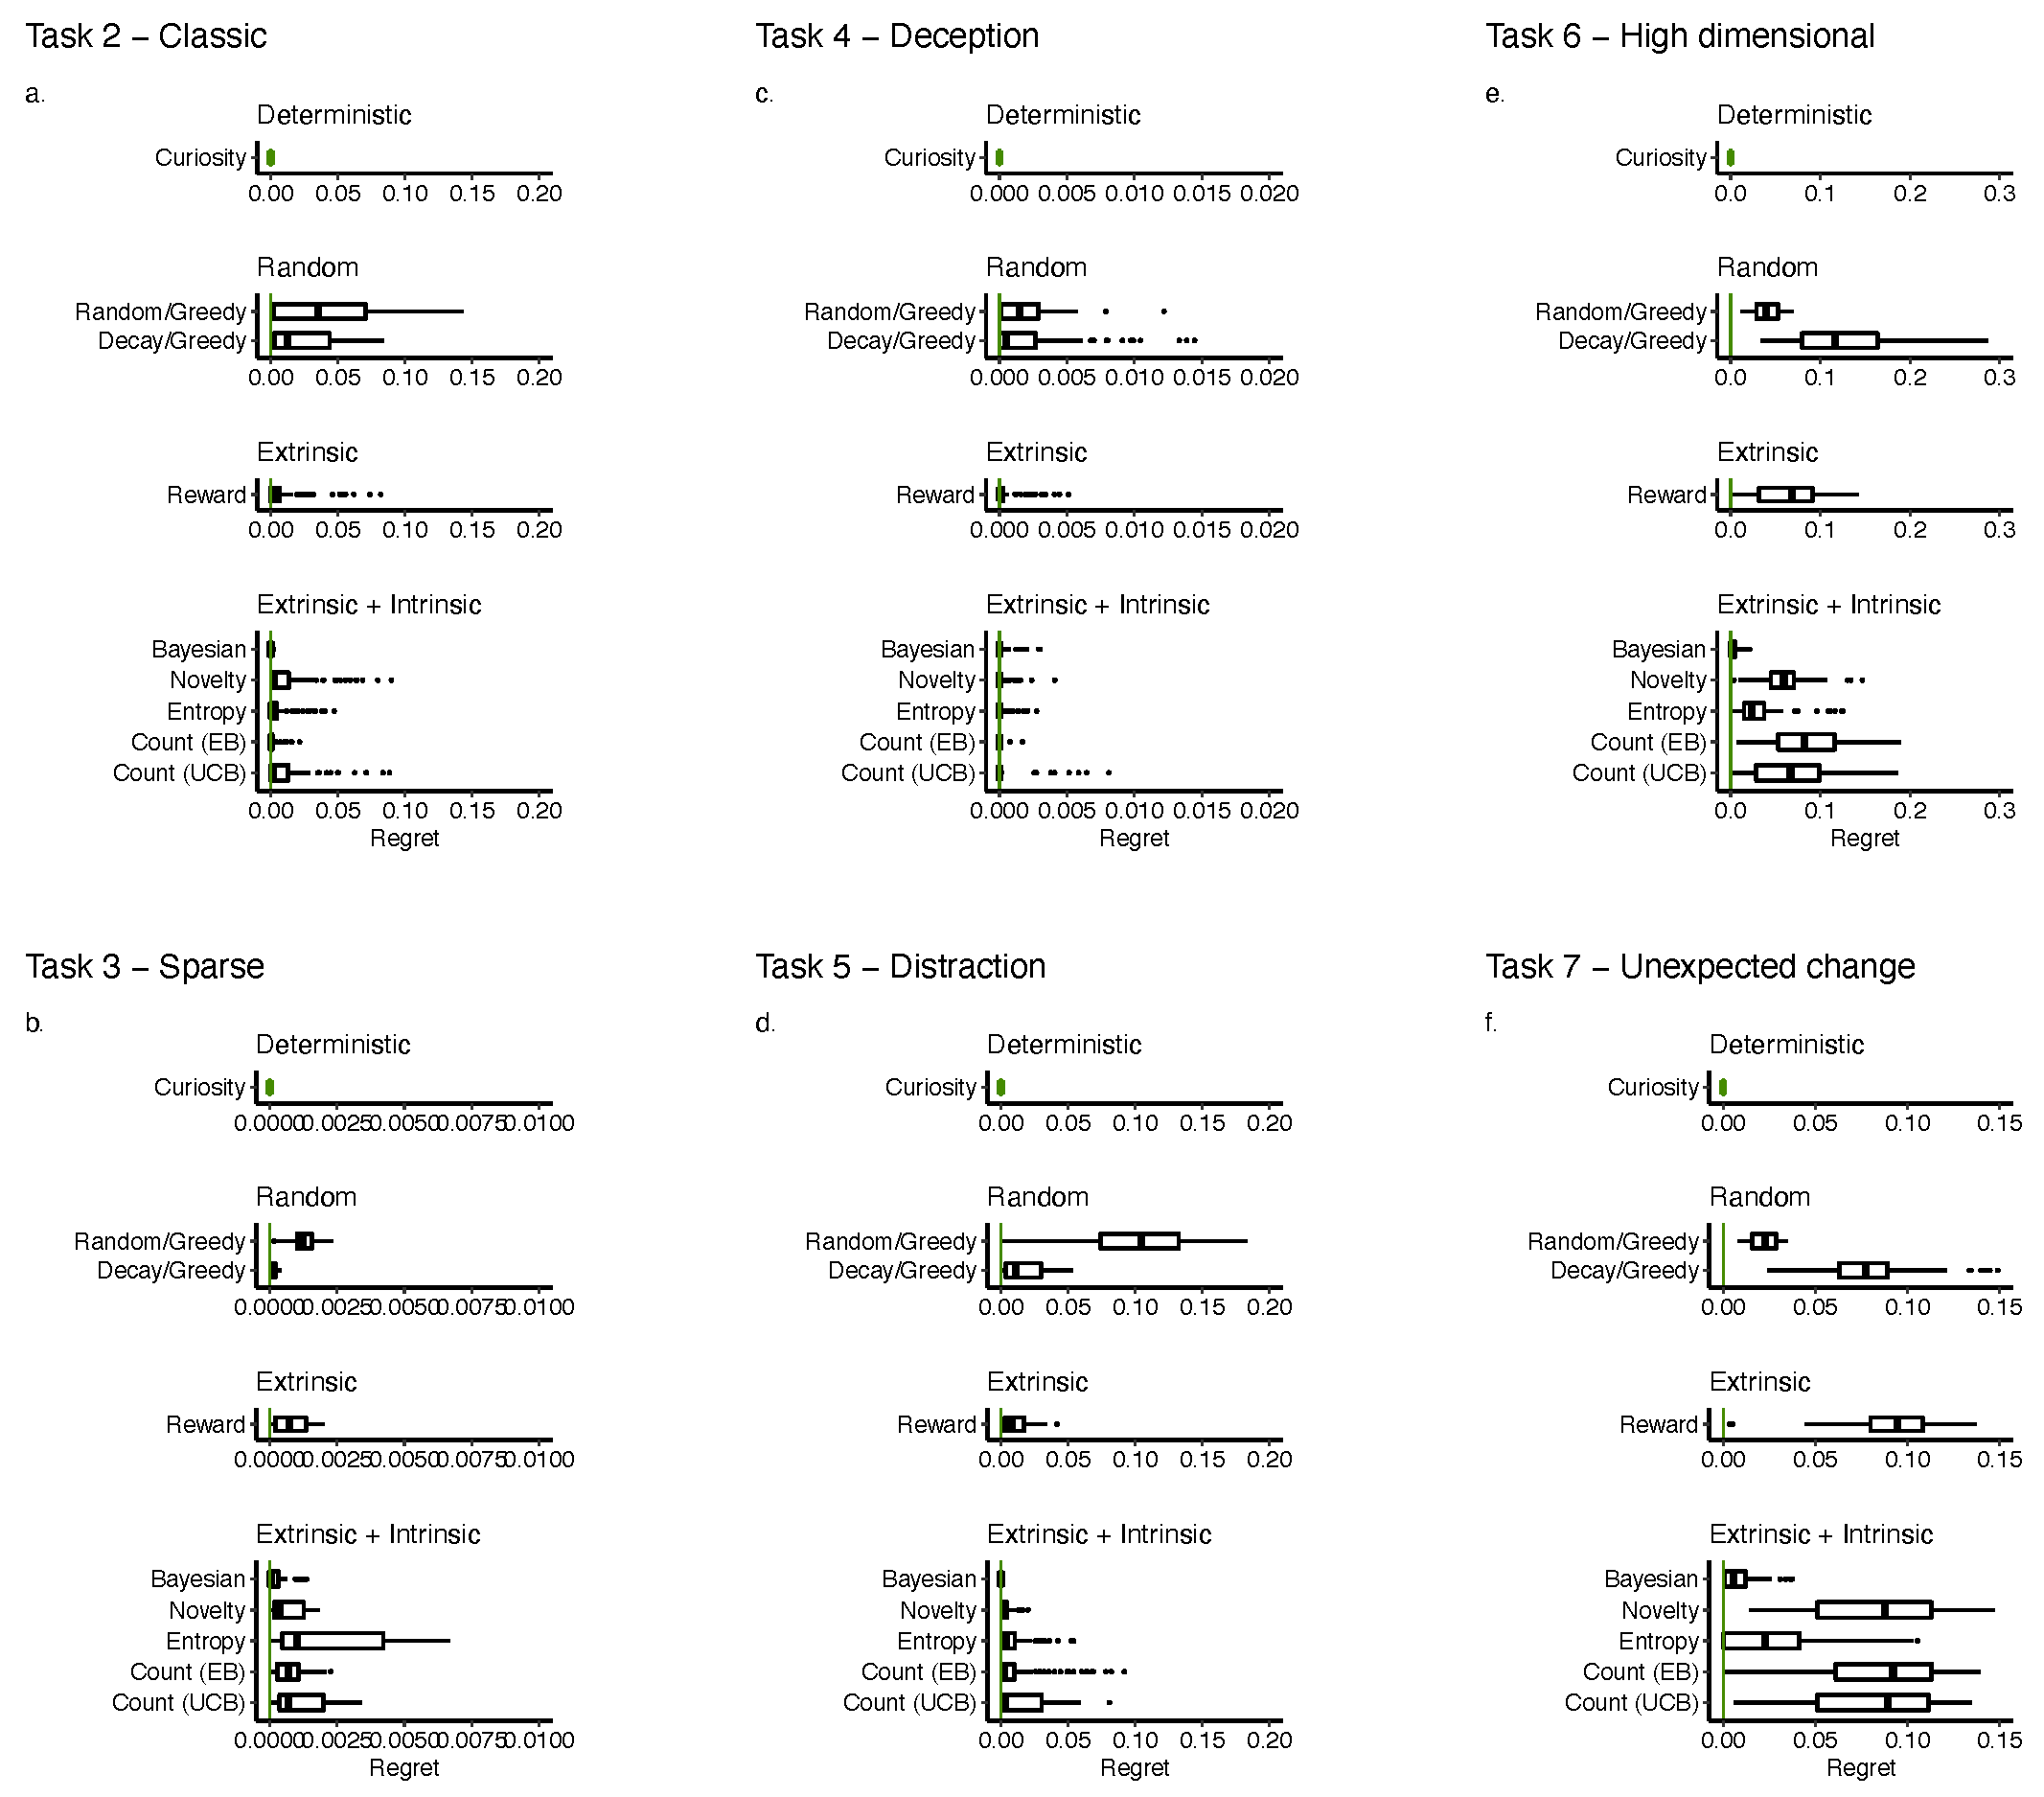
\includegraphics[width=1\linewidth]{img/supp_regret.pdf}}
	\figsupp{Summary of information value (\textit{Tasks 2-7})}{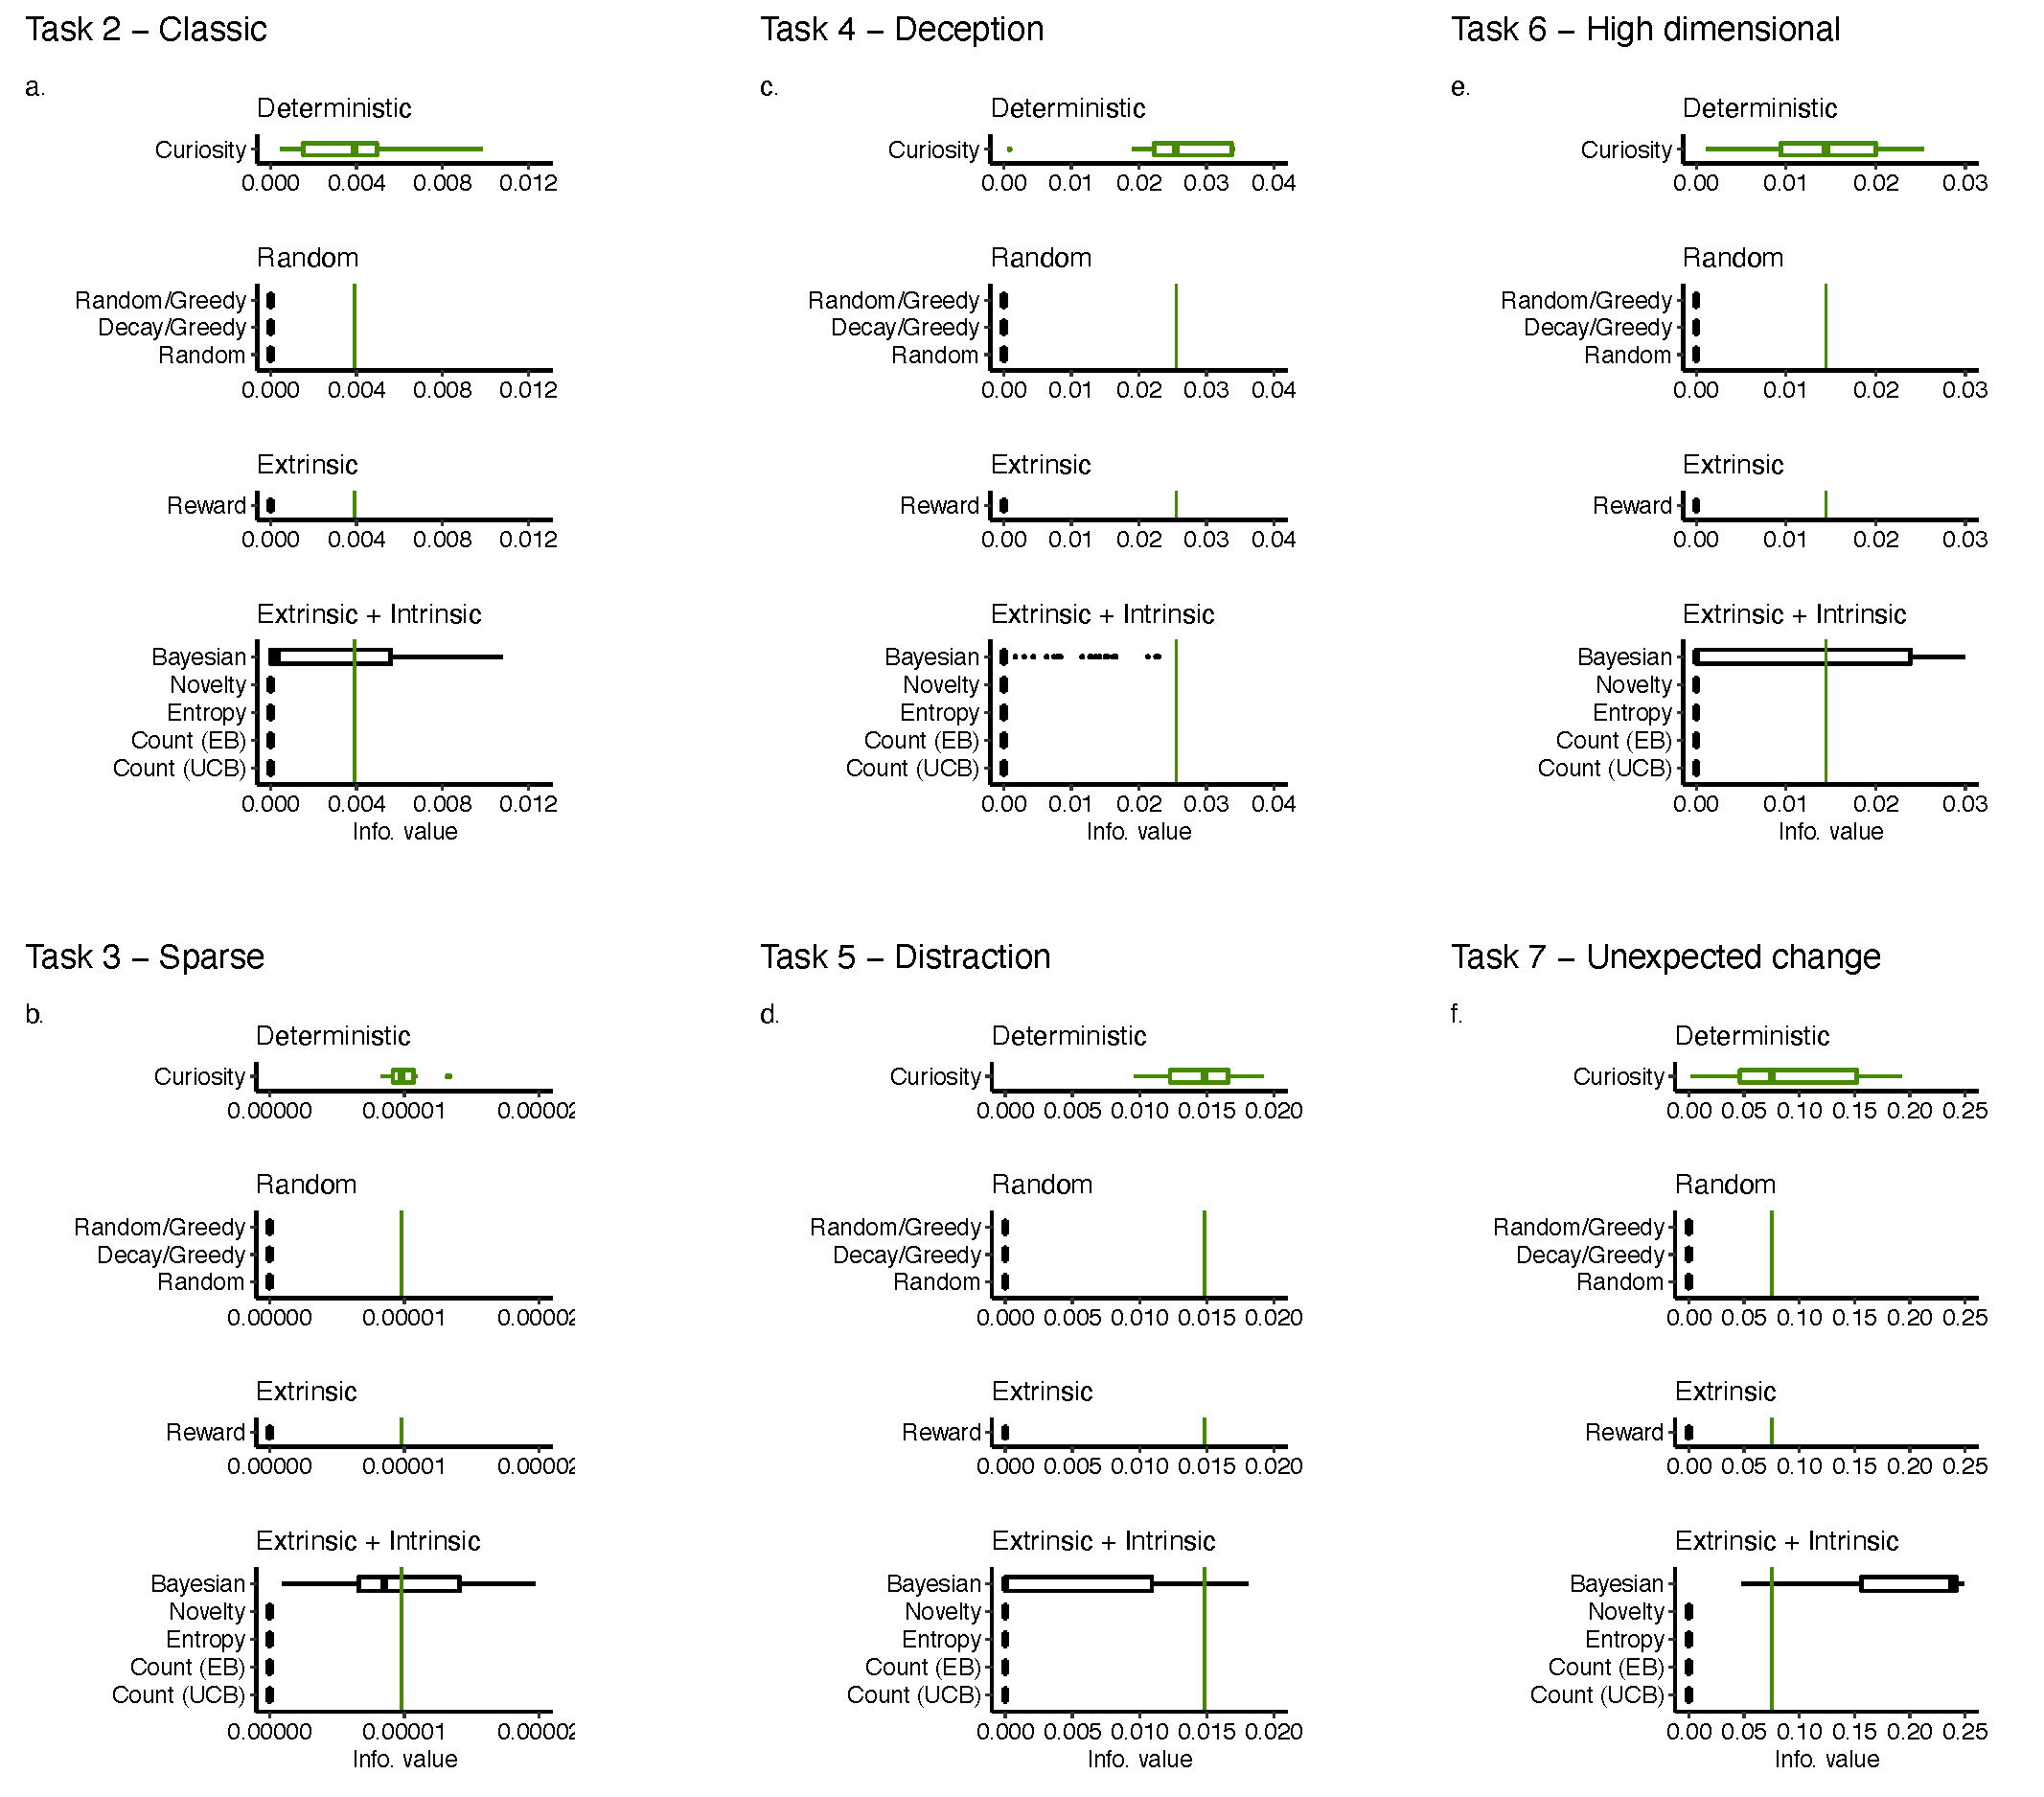
\includegraphics[width=1\linewidth]{img/supp_info.pdf}}
	\figsupp{Examples of exploration (Task 1). Here we simulated different sets of hyper-parameters on the same task and random seed. We view each parameter set as a unique ``animal'' \citep{Prescott2006}. So this figure estimates the degree and kind of variability we might expect in a natural experiment. }{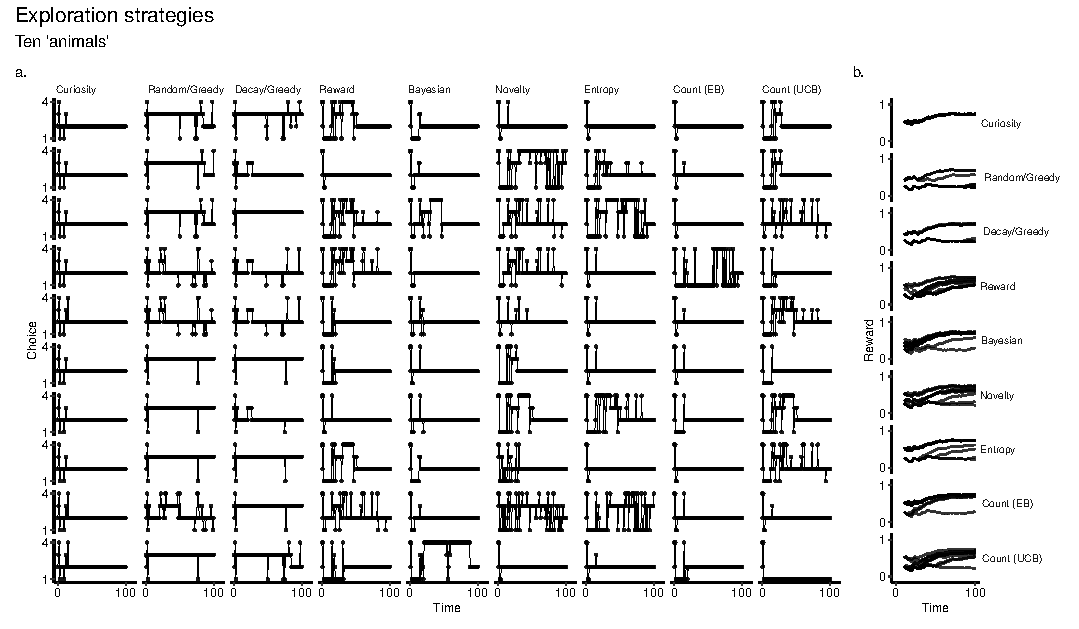
\includegraphics[width=1\linewidth]{img/exploration1.pdf}}
	\end{fullwidth}
\end{figure}

\textit{Task 1.} is an information gathering task, which we discussed already above. \textit{Task 2} was designed to examine reward collection, in probabilistic reward setting very common in the decision making literature \citep{schonberg2007reinforcement,frank2004carrot,cavanagh2014conflict,jahfari2019cross,collins2014opponent,collins2017interactions,glascher2010states}. Rewards were 0 or 1. The best choice had a payout of $p(R=1) = 0.8$. This is a much higher average payout than the others ($p(R=1) = 0.2$). At no point does the task generate symbolic information. See, Fig.~\ref{fig:payout1}\textbf{b}. 

The results for Task 1 were discussed above. As for Task 2, we expected all the exploration strategies to succeed. While this was indeed the case, our deterministic curiosity was the top-performer in terms of median rewards collected, though by a small margin (Fig~\ref{fig:summary}\textbf{a}).

\textit{Task 3.} was designed with very sparse rewards \citep{Mniha,Silver2016b,Silver2018} and there were 10 choices, making this a more difficult task (Fig.~\ref{fig:payout1}\textbf{c}). Sparse rewards are a common problem in the natural world, where an animal may have to travel and search between each meal This is a difficult but not impossible task for vertebrates \citep{anderson1984optimal} and invertebrates \citep{westphal2006foraging}. That being said, most reinforcement learning algorithms will struggle in this setting because the thing they need to learn, that is rewards, are often absent. In this task we saw quite a bit more variation in performance, with the novelty-bonus strategy taking the top slot (this is the only time it does so).

\textit{Task 4.} was designed with deceptive rewards. By deceptive we mean that the best long-term option presents itself initially with a decreasing reward value (Fig.~\ref{fig:payout1}\textbf{d}). Such small deceptions abound in many natural contexts where one must often make short-term sacrifices \citep{internicola2012bumble}. It is well known that classic reinforcement learning will often struggle in this kind of task \citep{Lehman2011a,Sutton2018}. Here our deterministic curiosity is the only strategy that reaches above chance performance. Median performance of all other strategies are similar to the random control (Fig~\ref{fig:summary}\textbf{c}). 

\textit{Task 5} was designed to fool curiosity, our algorithm, by presenting information that was utterly irrelevant to reward collection, but had very high entropy and so ``interesting'' to our algorithm. We fully anticipated that this context would fool just our algorithm, with all other strategies performing well since they are largely agnostic to entropy. However, despite being designed to fail, deterministic curiosity still produced a competitive performance to the other strategies (Fig~\ref{fig:summary}\textbf{d}). 

\textit{Tasks 6-7} were designed as a pair, with both having 121 choices, and a complex payout structure. Tasks of this size are at the limit of human performance \citep{Wu2018}. We first trained all learners on \textit{Task 6}, then tested them in Task 7 which identical to 6, except the best payout arm is reset to be worst (Fig.~\ref{fig:payout1}\textbf{e}-\textbf{f}). In other words Tasks 6 and 7 were joined to measure learning in a high dimensional, but shifting, environments.

In Task 6 deterministic curiosity performed well, securing a second place finish. We note the Bayesian strategy  outperformed our approach. However, under the sudden non-stationarity in reward when switching tasks, the top Bayesian model became the worst on Task 7, and deterministic curiosity took the top spot. Compare Fig.~\ref{fig:summary}\textbf{e} to \textbf{f}. This is the robustness that we'd expect for any curiosity algorithm, whose main goal is to learn everything unbiased by other objectives. The environment and the objectives do change in real life, and so we must be prepared for this. Note how the other less-biased-toward-reward-value exploration models (count-based, novelty, and entropy models) also saw gains, to a lesser degree.

\subsubsection*{Robustness}
A good choice of boredom $eta$ is critical for our definition of curiosity, and was optimized carefully. We show an example of this importance in Fig.~\ref{fig:boredom2}. On the left hand side we did a random search over 10000 possible parameters to find a value for $\eta$ that produced excellent results. (This was the same kind of search we did to achieve the results shown in Fig. ~\ref{fig:summary}. On the right hand side we choose a value for boredom we knew would lead to a poor relative result. We then ran the 100 different randomly generated simulations which gives us the results seen in Fig.~\ref{fig:boredom2}). 

Carefully optimized boredom converged far more quickly (Fig.~\ref{fig:boredom2}a-b), generating more reward over time (Fig.~\ref{fig:boredom2}c-d), and showed far more in consistency during exploration (Fig.~\ref{fig:boredom2}e-f). 

These experiments in setting $\eta$ are also useful in demonstrating the wide variance in behavior that is possible with a deterministic search. Exploration in these figures is deterministic, as prescribed by Eq.~\ref{eq:meta_greedy}. The environment was stochastic however and so the variations come from the environment changing what is learned, which then changes what the best learner should choose to learn next. 

\begin{figure}
	\begin{fullwidth}
	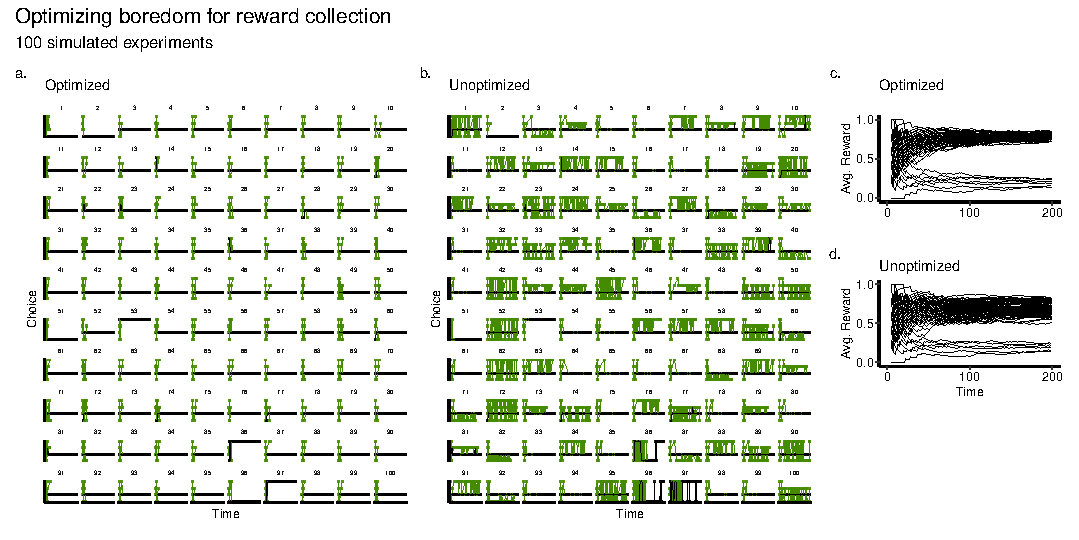
\includegraphics[width=1.0\linewidth]{img/boredom2.pdf} 
	\caption{The importance of boredom during reward collection (Task 2). One hundred example experiments, each began with a different random seed. 
	\textbf{a}. Behavioral choices with optimized boredom.
	\textbf{b}. Behavioral choices with unoptimized boredom.
	\textbf{c,d}. Average reward as a function of time for optimized (c) and unoptimized (d) boredom.
	}
	\label{fig:boredom2} 
	\end{fullwidth}
\end{figure}

Unlike idealised simulations, animals cannot pre-optimize their search parameters for every task. We therefore explored reward collection as a function of 1000 randomly chosen model parameters, and reexamined performance on Tasks 1 and 7=6. These were chosen to represent an ``easy'' task, and a ``hard one''. These results are shown in Fig.~\ref{fig:robust}. 

As we observed in our other model comparisons, exploitation by deterministic curiosity produced top-3 performance on both tasks (Fig.~\ref{fig:robust}a-b). Most interesting is the performance for the worst parameters. Here deterministic curiosity was markedly better, with substantially less variability across different parameter schemes. We can explain this in the following way. All the other exploration strategies use parameters to tune the degree of exploration. With deterministic curiosity, however, we tune only when exploration should stop. The degree of exploration, the measure by how close it is to maximum entropy, is fixed by the model itself. It seems that here at least it is far more robust to tune the stopping point, rather than the degree of exploration.

\begin{figure}
	\begin{fullwidth}
	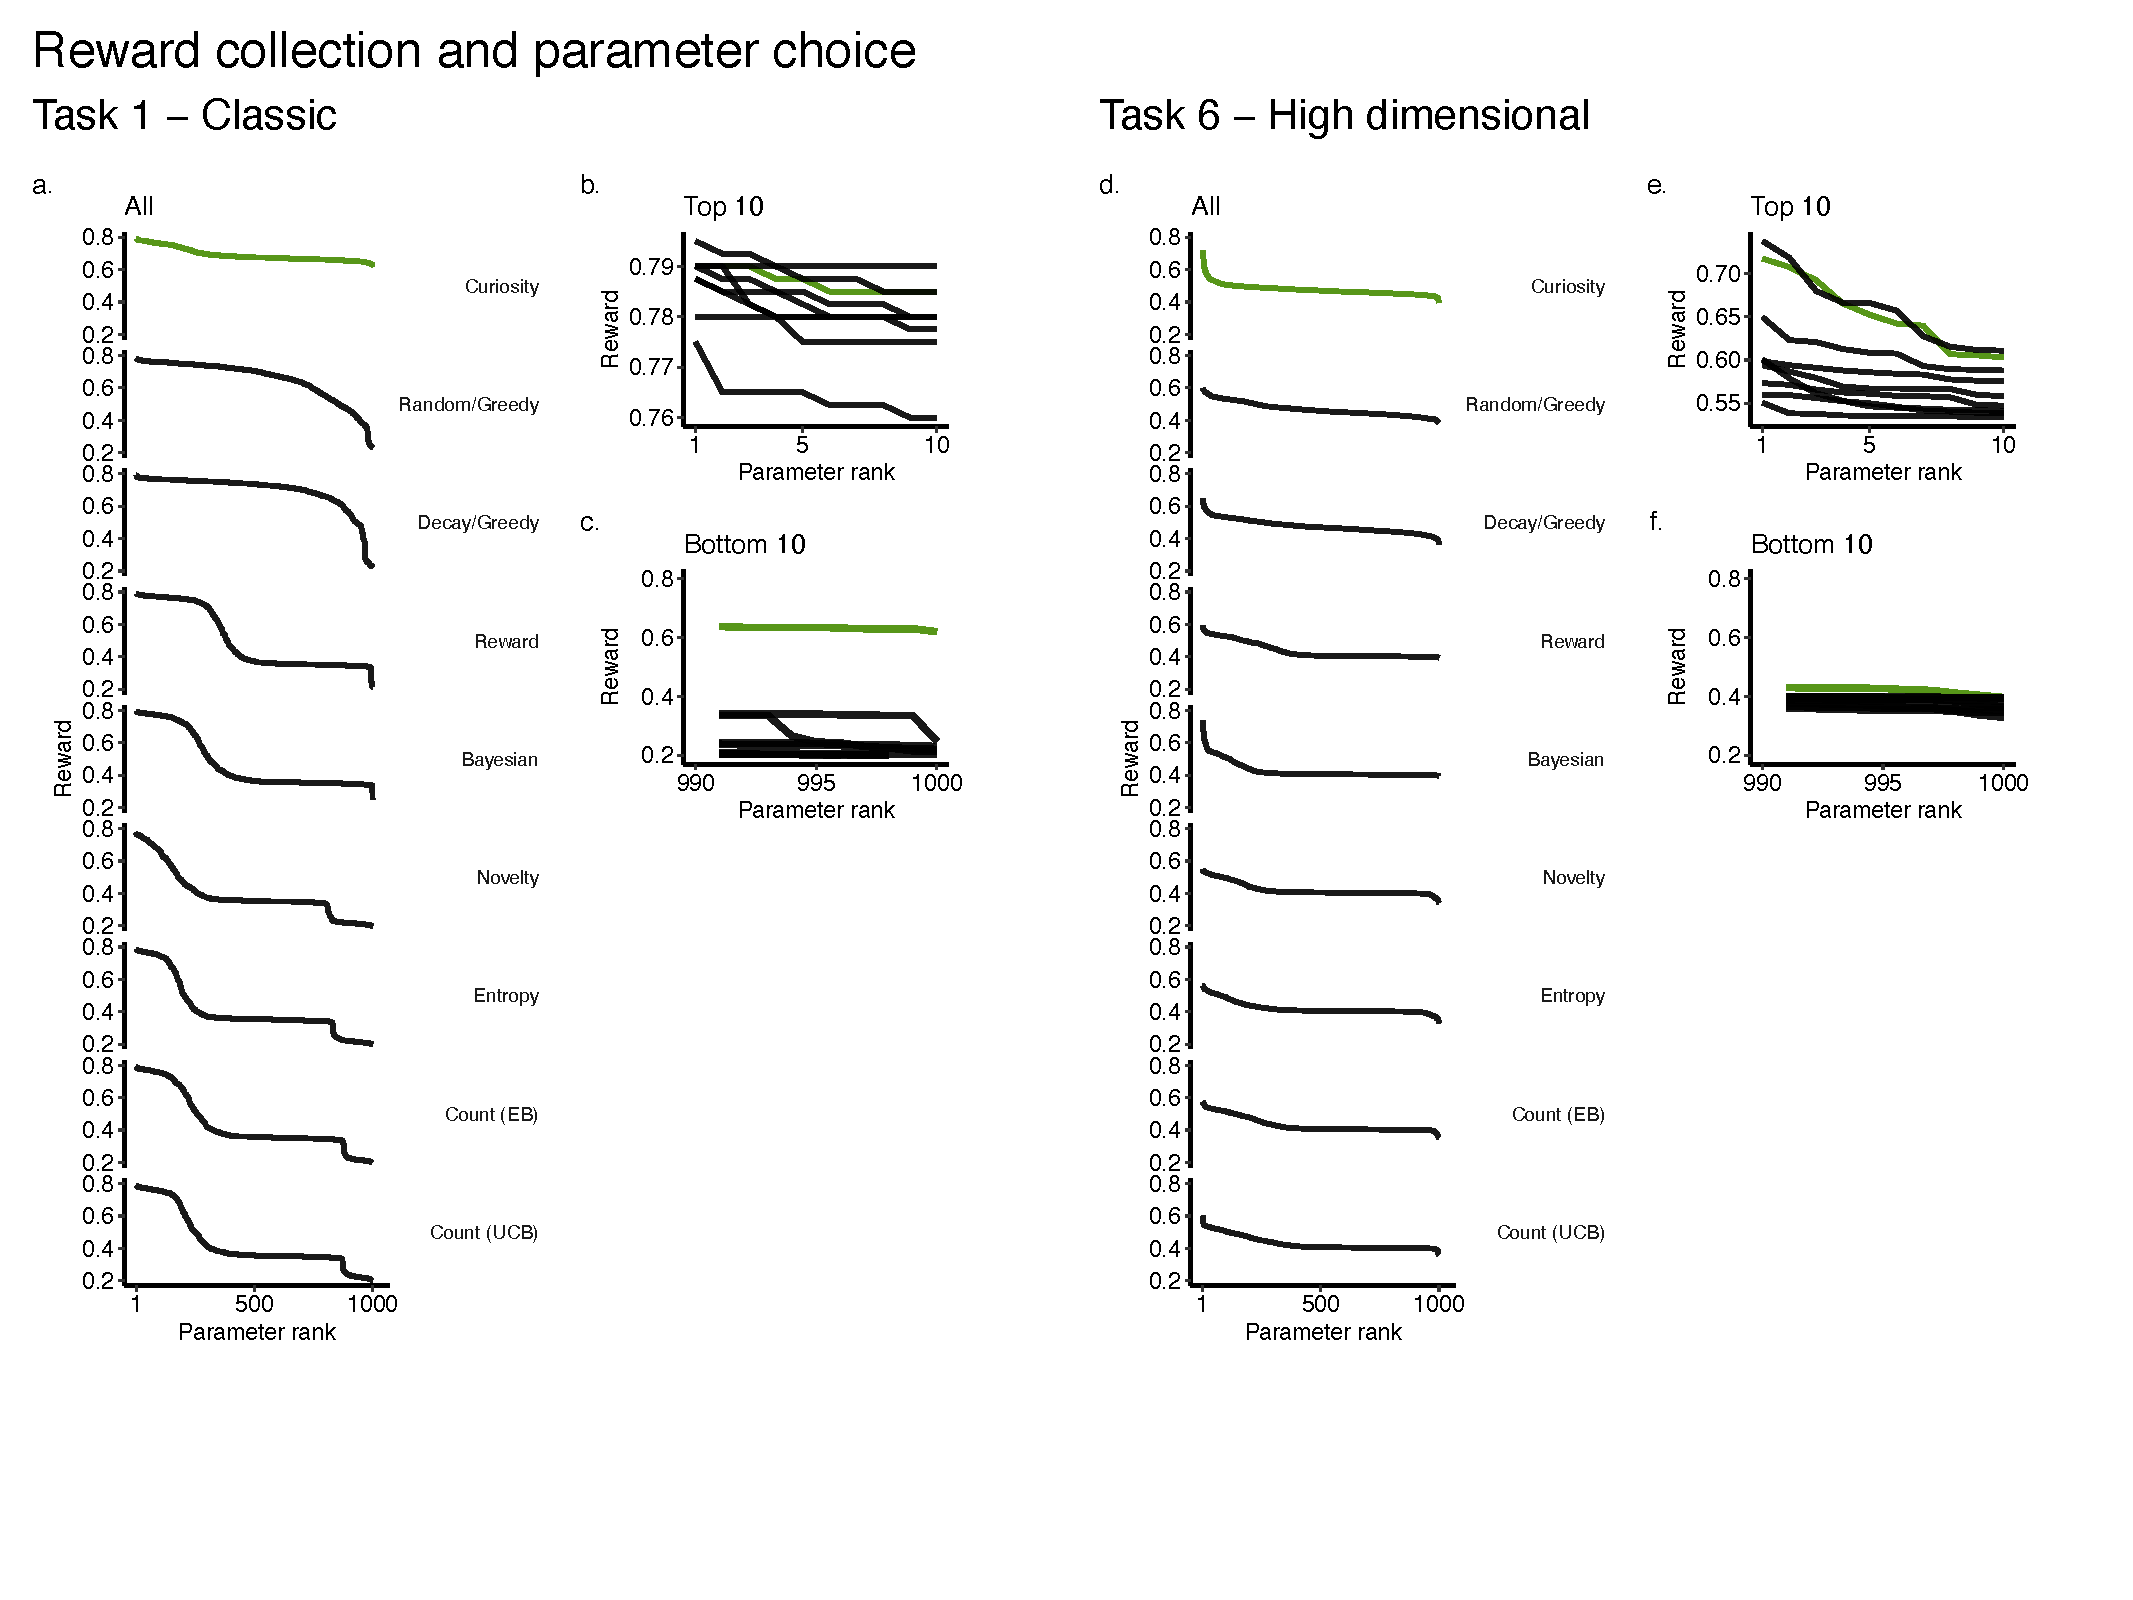
\includegraphics[width=1\linewidth]{img/robust.pdf} 
	\caption{Parameter selection and search performance (\textit{Task 2} and \textit{6}). We wanted to evaluate how robust performance was to poor and random hyperparameters. A very robustness exploration algorithm would produce strong performance with both the best parameter choices, and the worst parameter choices.   
	\textbf{a,d} Total reward for 1000 search hyperparameters, for each of strategies we considered.  
	\textbf{b,e} Performance with the top 10 hyperparameters, curiosity (green) compared to all the others.
	\textbf{c.f} Performance with the bottom 10 hyperparameters.
	}
	\figsupp{Adding noise to deterministic curiosity does degrade its performance. In this example control we added two levels of random noise. This only served to increase variability of convergence (a-c) and reduce the total rewards collected (d). Note: decision noise was modelled by sampling a Boltzmann distribution, as described in the \textit{Methods}.
    }{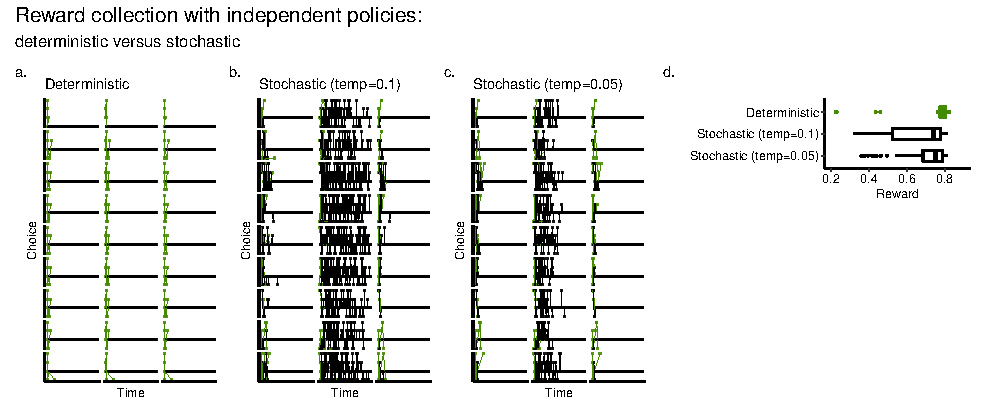
\includegraphics[width=1\linewidth]{img/independent2.pdf}}
    \figsupp{Noise across strategies. Adding noise to degrades performance to nearly the same degree (Task 2).
    }{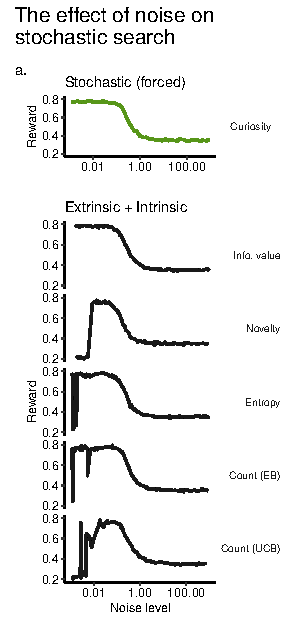
\includegraphics[width=0.95\linewidth]{img/forced2.pdf}}
	\label{fig:robust}
	\end{fullwidth}
\end{figure}
